\documentclass[11pt,a4paper]{report}

% Packages
\usepackage[utf8]{inputenc}
\usepackage[T1]{fontenc}
\usepackage{libertinus}            % Modern clean serif font
\usepackage{libertinust1math}      % Matching math font
\usepackage[scaled=0.85]{FiraMono} % Clean monospace for code listings
\usepackage{geometry}
\usepackage{graphicx}
\usepackage{xcolor}
\usepackage{listings}
\usepackage{hyperref}
\usepackage{booktabs}
\usepackage{longtable}
\usepackage{fancyhdr}
\usepackage{titlesec}
\usepackage{tocloft}
\usepackage{enumitem}
\usepackage{tikz}
\usetikzlibrary{shapes.geometric, arrows.meta, positioning, fit, backgrounds, calc, decorations.pathreplacing}
\usepackage{float}
\usepackage{caption}
\usepackage{subcaption}
\usepackage{multirow}
\usepackage{array}
\usepackage{tabularx}
\usepackage{fancyvrb}
\usepackage{mdframed}
\usepackage{tcolorbox}

% Page geometry
\geometry{
    top=1in,
    bottom=1in,
    left=1in,
    right=1in,
    headheight=14pt
}

% Colors
\definecolor{pittblue}{RGB}{0, 53, 148}
\definecolor{pittgold}{RGB}{255, 184, 28}
\definecolor{codegreen}{RGB}{0, 128, 0}
\definecolor{codegray}{RGB}{128, 128, 128}
\definecolor{codepurple}{RGB}{128, 0, 128}
\definecolor{backcolour}{RGB}{245, 245, 245}
\definecolor{terminalblack}{RGB}{30, 30, 30}
\definecolor{terminalgreen}{RGB}{0, 255, 0}
\definecolor{jetsongreen}{RGB}{118, 185, 0}
\definecolor{arduinoblue}{RGB}{0, 151, 156}

% Hyperref setup
\hypersetup{
    colorlinks=true,
    linkcolor=pittblue,
    filecolor=pittblue,
    urlcolor=pittblue,
    citecolor=pittblue,
    pdftitle={URC Complete Documentation},
    pdfauthor={University of Pittsburgh Robotics Club},
}

% Define YAML language for listings
\lstdefinelanguage{yaml}{
  keywords={true,false,null,y,n},
  sensitive=false,
  comment=[l]{\#},
  morecomment=[s]{/*}{*/},
  morestring=[b]',
  morestring=[b]"
}

% Code listing style
\lstdefinestyle{codestyle}{
    backgroundcolor=\color{backcolour},
    commentstyle=\color{codegreen},
    keywordstyle=\color{pittblue}\bfseries,
    numberstyle=\tiny\color{codegray},
    stringstyle=\color{codepurple},
    basicstyle=\ttfamily\footnotesize,
    breakatwhitespace=false,
    breaklines=true,
    captionpos=b,
    keepspaces=true,
    numbers=left,
    numbersep=5pt,
    showspaces=false,
    showstringspaces=false,
    showtabs=false,
    tabsize=2,
    frame=single,
    rulecolor=\color{pittblue},
}

\lstdefinestyle{terminal}{
    backgroundcolor=\color{terminalblack},
    basicstyle=\ttfamily\footnotesize\color{white},
    breaklines=true,
    frame=single,
    rulecolor=\color{codegray},
}

\lstset{style=codestyle}

% Custom box for important notes
\tcbuselibrary{skins,breakable}
\newtcolorbox{importantbox}{
    colback=pittgold!10,
    colframe=pittgold,
    title=Important,
    fonttitle=\bfseries,
    breakable,
}

\newtcolorbox{warningbox}{
    colback=red!10,
    colframe=red!70,
    title=Warning,
    fonttitle=\bfseries,
    breakable,
}

\newtcolorbox{tipbox}{
    colback=green!10,
    colframe=green!50!black,
    title=Tip,
    fonttitle=\bfseries,
    breakable,
}

% Header and footer
\pagestyle{fancy}
\fancyhf{}
\fancyhead[L]{\leftmark}
\fancyhead[R]{URC Documentation}
\fancyfoot[C]{\thepage}
\renewcommand{\headrulewidth}{0.4pt}
\renewcommand{\footrulewidth}{0.4pt}

% Title formatting
\titleformat{\chapter}[display]
    {\normalfont\huge\bfseries\color{pittblue}}
    {\chaptertitlename\ \thechapter}{20pt}{\Huge}

\titleformat{\section}
    {\normalfont\Large\bfseries\color{pittblue}}
    {\thesection}{1em}{}

\titleformat{\subsection}
    {\normalfont\large\bfseries\color{pittblue!80}}
    {\thesubsection}{1em}{}

% Document info
\title{
    \vspace{-2cm}
    % \includegraphics[width=0.3\textwidth]{logo.png}\\ % Uncomment when logo file is available
    \vspace{1cm}
    {\color{pittblue}\Huge\bfseries University Rover Challenge}\\
    \vspace{0.5cm}
    {\color{pittblue!70}\LARGE Complete Technical Documentation}\\
    \vspace{0.5cm}
    {\large\color{pittgold} \& Startup Guide}
}
\author{
    \textbf{University of Pittsburgh Robotics Club}\\
    \vspace{0.5cm}
    \small ROS 2 Humble $\bullet$ NVIDIA Jetson Nano $\bullet$ Docker
}
\date{Version 2.0 --- January 2026}

\begin{document}

% Title page
\maketitle
\thispagestyle{empty}

\vfill
\begin{center}
\begin{tabular}{ll}
\textbf{Platform:} & ROS 2 Humble Hawksbill \\
\textbf{Hardware:} & NVIDIA Jetson Nano, Arduino \\
\textbf{Deployment:} & Docker Containers \\
\textbf{GUI:} & PyQt5 \\
\end{tabular}
\end{center}

\newpage

% Table of Contents
\tableofcontents
\newpage

% List of Figures and Tables
\listoffigures
\listoftables
\newpage

%=============================================================================
\chapter{Project Overview}
\label{chap:overview}
%=============================================================================

\section{Introduction}

This document provides comprehensive technical documentation for the University of Pittsburgh Robotics Club's University Rover Challenge (URC) rover system. The system integrates advanced robotics technologies including:

\begin{itemize}
    \item \textbf{6-wheel differential drive system} with GoBilda motors
    \item \textbf{Multi-sensor fusion} including GPS, IMU, ultrasonic sensors, and cameras
    \item \textbf{ROS 2 Humble} for distributed robot communication
    \item \textbf{Docker containerization} for reproducible deployments
    \item \textbf{PyQt5 GUI system} for teleoperation and monitoring
\end{itemize}

\section{Competition Tasks}

The University Rover Challenge consists of multiple mission types:

\begin{table}[H]
\centering
\caption{URC Competition Tasks}
\begin{tabular}{@{}lp{10cm}@{}}
\toprule
\textbf{Task} & \textbf{Description} \\
\midrule
Autonomous Navigation & GPS-guided traversal of challenging Martian-analog terrain \\
Equipment Servicing & Precise manipulation tasks using robotic arm \\
Extreme Delivery & Package delivery in harsh environmental conditions \\
Science Operations & Sample collection and in-field analysis \\
Teleoperation & Manual control for complex scenarios \\
\bottomrule
\end{tabular}
\end{table}

\section{Key Specifications}

\begin{table}[H]
\centering
\caption{Rover System Specifications}
\begin{tabular}{@{}ll@{}}
\toprule
\textbf{Metric} & \textbf{Value} \\
\midrule
Navigation Accuracy & $\pm$2m GPS positioning \\
Video Latency & $<$200ms streaming \\
Control Response & $<$50ms command execution \\
Battery Life & 4+ hours autonomous operation \\
Operating Range & 1km+ radio communication \\
Motor Control & 6 GoBilda motors (0--255 PWM) \\
Camera Frame Rate & 30 Hz \\
IMU Update Rate & 10 Hz \\
Serial Baud Rate & 115200 bps \\
\bottomrule
\end{tabular}
\end{table}

\section{How Systems Work Together}

The URC rover system follows a distributed architecture where components work together through a multi-layered communication stack. Understanding this flow is essential for developers extending or debugging the system.

\subsection{End-to-End Data Flow}

When an operator interacts with the system, data flows through the following path:

\begin{enumerate}
    \item \textbf{User Input} --- Operator presses a key or moves a joystick on the base station
    \item \textbf{GUI Publisher} --- PyQt5 GUI captures input and calls \texttt{MotorPublisher.publish\_motor\_command()} or \texttt{TwistPublisher.publish\_twist()}
    \item \textbf{ROS 2 Topic} --- Publisher sends message to topic (e.g., \texttt{/motor\_control\_input} or \texttt{/cmd\_vel}) over WiFi via ROS 2 DDS
    \item \textbf{Bridge Subscriber} --- \texttt{MotorBridge} on Jetson receives message via subscription callback
    \item \textbf{Serial Transmission} --- Bridge formats command as comma-separated string and writes to Arduino via \texttt{serial.write()} at 115200 baud
    \item \textbf{Arduino Processing} --- Arduino firmware parses command, calculates differential drive values
    \item \textbf{Motor Control} --- Arduino sets PWM and direction pins to drive GoBilda motors
\end{enumerate}

\begin{figure}[H]
\centering
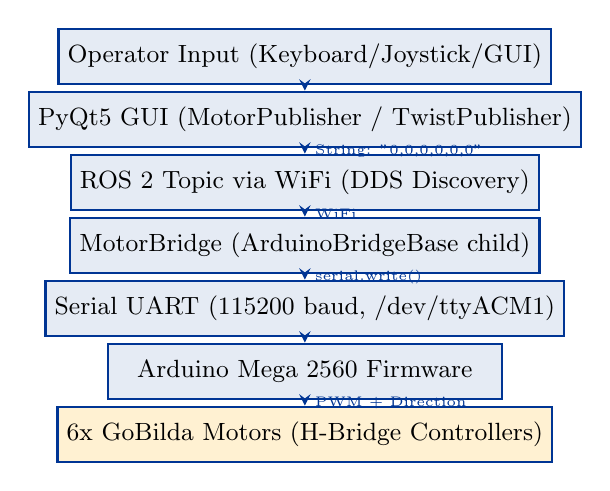
\begin{tikzpicture}[
    node distance=0.8cm,
    box/.style={rectangle, draw=pittblue, thick, minimum width=5cm, minimum height=0.7cm, align=center, fill=pittblue!10, font=\small},
    arrow/.style={->, thick, >=stealth, pittblue}
]
    \node[box] (input) {Operator Input (Keyboard/Joystick/GUI)};
    \node[box, below of=input] (gui) {PyQt5 GUI (MotorPublisher / TwistPublisher)};
    \node[box, below of=gui] (topic) {ROS 2 Topic via WiFi (DDS Discovery)};
    \node[box, below of=topic] (bridge) {MotorBridge (ArduinoBridgeBase child)};
    \node[box, below of=bridge] (serial) {Serial UART (115200 baud, /dev/ttyACM1)};
    \node[box, below of=serial] (arduino) {Arduino Mega 2560 Firmware};
    \node[box, below of=arduino, fill=pittgold!20] (motors) {6x GoBilda Motors (H-Bridge Controllers)};

    \draw[arrow] (input) -- (gui);
    \draw[arrow] (gui) -- node[right, font=\tiny] {String: "0,0,0,0,0,0"} (topic);
    \draw[arrow] (topic) -- node[right, font=\tiny] {WiFi} (bridge);
    \draw[arrow] (bridge) -- node[right, font=\tiny] {serial.write()} (serial);
    \draw[arrow] (serial) -- (arduino);
    \draw[arrow] (arduino) -- node[right, font=\tiny] {PWM + Direction} (motors);
\end{tikzpicture}
\caption{Complete Motor Control Data Flow --- Note: \texttt{/dev/ttyACM1} assignment requires Motor Arduino to be plugged in \textbf{second}. See Section~\ref{sec:usb-enumeration} for required plug-in order.}
\end{figure}

\begin{importantbox}
\textbf{Hardware Requirement: Two Arduino Boards}

This system requires \textbf{two separate Arduino boards}:
\begin{enumerate}
    \item \textbf{Sensor Arduino} (plugged in first $\rightarrow$ \texttt{/dev/ttyACM0}) --- Runs IMU, GPS, and ultrasonic sensor firmware
    \item \textbf{Motor Arduino} (plugged in second $\rightarrow$ \texttt{/dev/ttyACM1}) --- Runs motor control firmware for 6-wheel drive
\end{enumerate}

The port numbers are assigned based on USB plug-in order, not physical port location. See Section~\ref{sec:usb-enumeration} for detailed plug-in procedures.
\end{importantbox}

\subsection{Sensor Data Return Path}

Sensor data flows in the reverse direction:

\begin{enumerate}
    \item \textbf{Hardware Sensor} --- BNO055 IMU reads orientation, GPS receives NMEA sentences
    \item \textbf{Arduino} --- Formats sensor data and sends via \texttt{Serial.println()}
    \item \textbf{Bridge Timer} --- \texttt{ArduinoBridgeBase.read\_from\_arduino()} executes every 100ms via ROS 2 timer
    \item \textbf{ROS 2 Publisher} --- Bridge publishes data to topic (e.g., \texttt{/imu\_data}, \texttt{/gps\_data})
    \item \textbf{GUI Subscriber} --- \texttt{IMUSubscriber} or \texttt{GPSSubscriber} receives message, parses with data parser
    \item \textbf{PyQt5 Signal} --- Subscriber emits \texttt{imu\_data\_updated} signal with parsed values
    \item \textbf{GUI Update} --- Signal triggers slot function that updates UI labels/displays
\end{enumerate}

\subsection{Base Station vs. Rover Responsibilities}

\begin{table}[H]
\centering
\caption{Component Location and Purpose}
\begin{tabular}{@{}llp{7cm}@{}}
\toprule
\textbf{Component} & \textbf{Location} & \textbf{Responsibility} \\
\midrule
GUI Applications & Base Station & User interface, input capture, data visualization \\
Publisher Classes & Base Station & Convert user actions to ROS 2 messages \\
Subscriber Classes & Base Station & Receive sensor data, parse, update GUI \\
Data Parsers & Base Station & Parse raw sensor strings into usable values \\
\midrule
Bridge Classes & Rover (Jetson) & ROS 2 $\leftrightarrow$ Serial translation \\
Supervisor & Rover (Jetson) & Process management, auto-restart \\
Arduino Firmware & Rover (Arduino) & Hardware control, sensor reading \\
Motors/Sensors & Rover (Physical) & Physical actuation and sensing \\
\bottomrule
\end{tabular}
\end{table}

\begin{tipbox}
\textbf{When to modify each component:}
\begin{itemize}
    \item \textbf{Add new GUI control} $\rightarrow$ Modify/create Publisher class in \texttt{guis/publishers/}
    \item \textbf{Add new sensor display} $\rightarrow$ Create Subscriber class in \texttt{guis/subscribers/} with data parser
    \item \textbf{Change serial protocol} $\rightarrow$ Modify Bridge class in \texttt{ros\_bridge/} and corresponding Arduino sketch
    \item \textbf{Add new hardware} $\rightarrow$ Create new Bridge class inheriting from \texttt{ArduinoBridgeBase}
\end{itemize}
\end{tipbox}

%=============================================================================
\chapter{System Architecture}
\label{chap:architecture}
%=============================================================================

\section{Technology Stack}

The rover system leverages a modern technology stack for robotics development:

\begin{figure}[H]
\centering
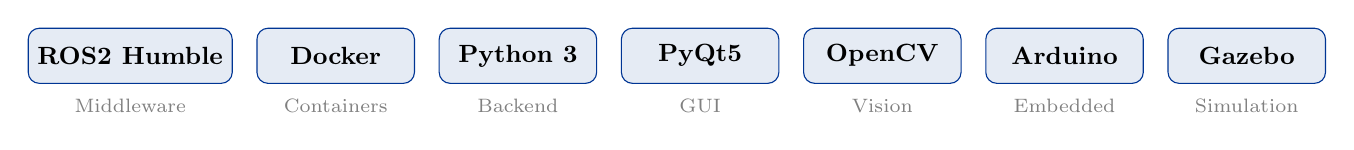
\begin{tikzpicture}[
    node distance=0.3cm,
    box/.style={rectangle, rounded corners, draw=pittblue, fill=pittblue!10, minimum width=2cm, minimum height=0.7cm, font=\small\bfseries},
    label/.style={font=\scriptsize, gray}
]
\node[box] (ros) {ROS2 Humble};
\node[box, right=of ros] (docker) {Docker};
\node[box, right=of docker] (python) {Python 3};
\node[box, right=of python] (pyqt) {PyQt5};
\node[box, right=of pyqt] (opencv) {OpenCV};
\node[box, right=of opencv] (arduino) {Arduino};
\node[box, right=of arduino] (gazebo) {Gazebo};

\node[label, below=2pt of ros] {Middleware};
\node[label, below=2pt of docker] {Containers};
\node[label, below=2pt of python] {Backend};
\node[label, below=2pt of pyqt] {GUI};
\node[label, below=2pt of opencv] {Vision};
\node[label, below=2pt of arduino] {Embedded};
\node[label, below=2pt of gazebo] {Simulation};
\end{tikzpicture}
\caption{Technology Stack}
\label{fig:tech-stack}
\end{figure}

\section{High-Level Architecture}

The rover system uses a \textbf{dual-container architecture} for optimal performance and separation of concerns.

\begin{figure}[H]
\centering
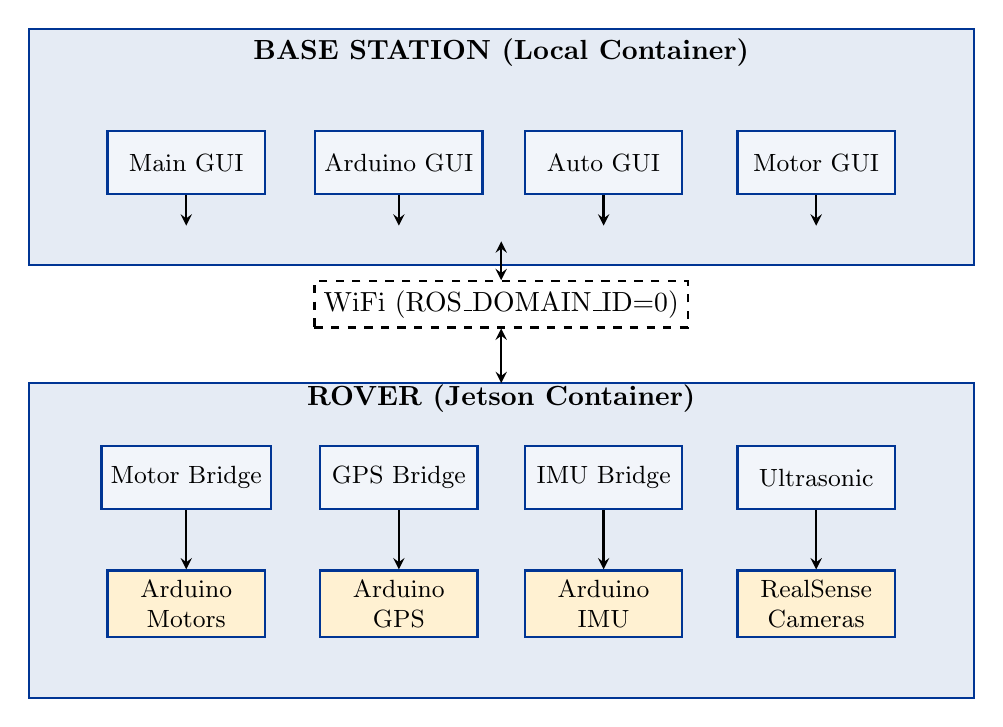
\begin{tikzpicture}[
    node distance=1.5cm,
    box/.style={rectangle, draw=pittblue, thick, minimum width=3cm, minimum height=1cm, align=center, fill=pittblue!10},
    smallbox/.style={rectangle, draw=pittblue, thick, minimum width=2cm, minimum height=0.8cm, align=center, fill=pittblue!5, font=\small},
    arrow/.style={->, thick, >=stealth}
]
    % Base Station
    \node[box, minimum width=12cm, minimum height=3cm] (base) at (0, 4) {};
    \node at (0, 5.2) {\textbf{BASE STATION (Local Container)}};

    \node[smallbox] (gui1) at (-4, 3.8) {Main GUI};
    \node[smallbox] (gui2) at (-1.3, 3.8) {Arduino GUI};
    \node[smallbox] (gui3) at (1.3, 3.8) {Auto GUI};
    \node[smallbox] (gui4) at (4, 3.8) {Motor GUI};

    % WiFi Connection
    \node[draw, dashed, thick, minimum width=3cm] (wifi) at (0, 2) {WiFi (ROS\_DOMAIN\_ID=0)};

    % Rover
    \node[box, minimum width=12cm, minimum height=4cm] (rover) at (0, -1) {};
    \node at (0, 0.8) {\textbf{ROVER (Jetson Container)}};

    \node[smallbox] (motor) at (-4, -0.2) {Motor Bridge};
    \node[smallbox] (gps) at (-1.3, -0.2) {GPS Bridge};
    \node[smallbox] (imu) at (1.3, -0.2) {IMU Bridge};
    \node[smallbox] (ultra) at (4, -0.2) {Ultrasonic};

    \node[smallbox, fill=pittgold!20] (arduino1) at (-4, -1.8) {Arduino\\Motors};
    \node[smallbox, fill=pittgold!20] (arduino2) at (-1.3, -1.8) {Arduino\\GPS};
    \node[smallbox, fill=pittgold!20] (arduino3) at (1.3, -1.8) {Arduino\\IMU};
    \node[smallbox, fill=pittgold!20] (camera) at (4, -1.8) {RealSense\\Cameras};

    % Arrows
    \draw[arrow] (gui1) -- ++(0, -0.8);
    \draw[arrow] (gui2) -- ++(0, -0.8);
    \draw[arrow] (gui3) -- ++(0, -0.8);
    \draw[arrow] (gui4) -- ++(0, -0.8);

    \draw[arrow, <->] (0, 2.8) -- (wifi);
    \draw[arrow, <->] (wifi) -- (0, 1);

    \draw[arrow] (motor) -- (arduino1);
    \draw[arrow] (gps) -- (arduino2);
    \draw[arrow] (imu) -- (arduino3);
    \draw[arrow] (ultra) -- (camera);

\end{tikzpicture}
\caption{System Architecture Overview}
\end{figure}

\section{Detailed Hardware Architecture}

The following diagram shows the complete hardware interconnections of the rover system, including power distribution, communication pathways, and all sensor subsystems.

\begin{figure}[H]
\centering
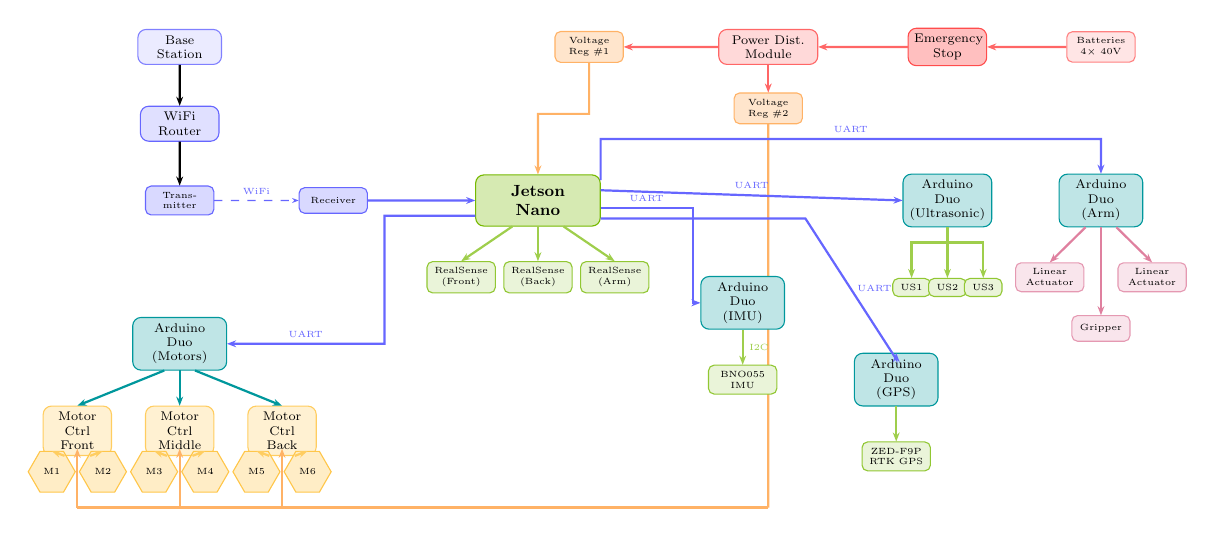
\begin{tikzpicture}[
    scale=0.65,
    transform shape,
    box/.style={rectangle, rounded corners=3pt, draw, minimum height=0.6cm, font=\scriptsize, align=center, text width=1.6cm},
    smallbox/.style={rectangle, rounded corners=2pt, draw, minimum height=0.5cm, font=\tiny, align=center, text width=1.1cm},
    motor/.style={regular polygon, regular polygon sides=6, draw=pittgold!80, fill=pittgold!25, minimum size=0.5cm, font=\tiny},
    sensor/.style={rectangle, rounded corners=2pt, draw=jetsongreen!80, fill=jetsongreen!15, minimum height=0.42cm, font=\tiny, text width=1.1cm, align=center},
    arr/.style={-{Stealth[scale=0.5]}, thick},
    darr/.style={-{Stealth[scale=0.5]}, dashed}
]

% === POWER SYSTEM (top, y=5) ===
\node[smallbox, fill=red!10, draw=red!50] (batt) at (10,5) {Batteries\\$4\times$ 40V};
\node[box, fill=red!25, draw=red!70, text width=1.3cm] (estop) at (7,5) {Emergency\\Stop};
\node[box, fill=red!15, draw=red!60, text width=1.7cm] (pdu) at (3.5,5) {Power Dist.\\Module};
\node[smallbox, fill=orange!20, draw=orange!60] (vreg1) at (0,5) {Voltage\\Reg \#1};

\draw[arr, red!60] (batt) -- (estop);
\draw[arr, red!60] (estop) -- (pdu);
\draw[arr, red!60] (pdu) -- (vreg1);

% V-Reg #2 (directly below PDU)
\node[smallbox, fill=orange!20, draw=orange!60] (vreg2) at (3.5,3.8) {Voltage\\Reg \#2};
\draw[arr, red!60] (pdu.south) -- (vreg2.north);

% === COMMUNICATION (left side) ===
\node[box, fill=blue!8, draw=blue!50, text width=1.4cm] (base) at (-8,5) {Base\\Station};
\node[box, fill=blue!12, draw=blue!60, text width=1.3cm] (router) at (-8,3.5) {WiFi\\Router};
\node[smallbox, fill=blue!15, draw=blue!60] (tx) at (-8,2) {Trans-\\mitter};
\node[smallbox, fill=blue!15, draw=blue!60] (rx) at (-5,2) {Receiver};

\draw[arr] (base) -- (router);
\draw[arr] (router) -- (tx);
\draw[darr, blue!60] (tx) -- node[above, font=\tiny] {WiFi} (rx);

% === JETSON NANO (center, y=2) ===
\node[box, fill=jetsongreen!30, draw=jetsongreen, text width=2.2cm, minimum height=1cm, font=\small\bfseries] (jetson) at (-1,2) {Jetson\\Nano};

% Rx to Jetson
\draw[arr, blue!60] (rx) -- (jetson);

% V-Reg #1 to Jetson
\draw[arr, orange!60] (vreg1.south) -- ++(0,-1) -- ++(-1,0) -- (jetson.north);

% === CAMERAS (y=0.5, below Jetson) ===
\node[sensor] (camf) at (-2.5,0.5) {RealSense\\(Front)};
\node[sensor] (camb) at (-1,0.5) {RealSense\\(Back)};
\node[sensor] (cama) at (0.5,0.5) {RealSense\\(Arm)};

\draw[arr, jetsongreen!70] (jetson.south) ++(-0.5,0) -- (camf.north);
\draw[arr, jetsongreen!70] (jetson.south) -- (camb.north);
\draw[arr, jetsongreen!70] (jetson.south) ++(0.5,0) -- (cama.north);

% === MOTOR ARDUINO (x=-8, y=-0.8) ===
\node[box, fill=arduinoblue!25, draw=arduinoblue, text width=1.6cm] (ardmotor) at (-8,-0.8) {Arduino Duo\\(Motors)};

% Jetson to Motor Arduino
\draw[arr, blue!60] (jetson.west) ++(0,-0.3) -- (-4,1.7) -- (-4,-0.8) -- node[above, font=\tiny] {UART} (ardmotor.east);

% === MOTOR CONTROLLERS (y=-2.5) ===
\node[box, fill=pittgold!20, draw=pittgold!70, text width=1.1cm] (mcf) at (-10,-2.5) {Motor Ctrl\\Front};
\node[box, fill=pittgold!20, draw=pittgold!70, text width=1.1cm] (mcm) at (-8,-2.5) {Motor Ctrl\\Middle};
\node[box, fill=pittgold!20, draw=pittgold!70, text width=1.1cm] (mcb) at (-6,-2.5) {Motor Ctrl\\Back};

\draw[arr, arduinoblue] (ardmotor.south) ++(-0.3,0) -- (mcf.north);
\draw[arr, arduinoblue] (ardmotor.south) -- (mcm.north);
\draw[arr, arduinoblue] (ardmotor.south) ++(0.3,0) -- (mcb.north);

% V-Reg #2 to Motor Controllers
\draw[orange!60, thick] (vreg2.south) -- (3.5,-4);
\draw[orange!60, thick] (3.5,-4) -- (-10,-4);
\draw[arr, orange!60] (-10,-4) -- (-10,-2.85);
\draw[arr, orange!60] (-8,-4) -- (-8,-2.85);
\draw[arr, orange!60] (-6,-4) -- (-6,-2.85);

% === MOTORS (y=-3.3) ===
\node[motor] (m1) at (-10.5,-3.3) {M1};
\node[motor] (m2) at (-9.5,-3.3) {M2};
\node[motor] (m3) at (-8.5,-3.3) {M3};
\node[motor] (m4) at (-7.5,-3.3) {M4};
\node[motor] (m5) at (-6.5,-3.3) {M5};
\node[motor] (m6) at (-5.5,-3.3) {M6};

\draw[arr, pittgold!70] (mcf.south) ++(-0.25,0) -- (m1.north);
\draw[arr, pittgold!70] (mcf.south) ++(0.25,0) -- (m2.north);
\draw[arr, pittgold!70] (mcm.south) ++(-0.25,0) -- (m3.north);
\draw[arr, pittgold!70] (mcm.south) ++(0.25,0) -- (m4.north);
\draw[arr, pittgold!70] (mcb.south) ++(-0.25,0) -- (m5.north);
\draw[arr, pittgold!70] (mcb.south) ++(0.25,0) -- (m6.north);

% === IMU ARDUINO (x=3, y=0) ===
\node[box, fill=arduinoblue!25, draw=arduinoblue, text width=1.4cm] (ardimu) at (3,0) {Arduino Duo\\(IMU)};
\node[sensor] (imu) at (3,-1.5) {BNO055\\IMU};

\draw[arr, blue!60] (jetson.east) ++(0,-0.15) -- node[above, font=\tiny] {UART} ++(1.8,0) |- (ardimu.west);
\draw[arr, jetsongreen!70] (ardimu.south) -- node[right, font=\tiny] {I2C} (imu.north);

% === GPS ARDUINO (x=6, y=-1.5) ===
\node[box, fill=arduinoblue!25, draw=arduinoblue, text width=1.4cm] (ardgps) at (6,-1.5) {Arduino Duo\\(GPS)};
\node[sensor] (gps) at (6,-3) {ZED-F9P\\RTK GPS};

\draw[arr, blue!60] (jetson.east) ++(0,-0.35) -- ++(4,0) -- node[right, font=\tiny] {UART} (6,-1.1) -- (ardgps.north);
\draw[arr, jetsongreen!70] (ardgps.south) -- (gps.north);

% === ULTRASONIC ARDUINO (x=7, y=2) ===
\node[box, fill=arduinoblue!25, draw=arduinoblue, text width=1.5cm] (ardus) at (7,2) {Arduino Duo\\(Ultrasonic)};

\draw[arr, blue!60] (jetson.east) ++(0,0.2) -- node[above, font=\tiny] {UART} (ardus.west);

% Ultrasonic sensors (3 sensors)
\node[sensor, text width=0.5cm, minimum height=0.25cm] (us1) at (6.3,0.3) {US1};
\node[sensor, text width=0.5cm, minimum height=0.25cm] (us2) at (7,0.3) {US2};
\node[sensor, text width=0.5cm, minimum height=0.25cm] (us3) at (7.7,0.3) {US3};

\draw[arr, jetsongreen!70] (ardus.south) -- ++(0,-0.3) -| (us1.north);
\draw[arr, jetsongreen!70] (ardus.south) -- ++(0,-0.3) -| (us2.north);
\draw[arr, jetsongreen!70] (ardus.south) -- ++(0,-0.3) -| (us3.north);

% === ARM ARDUINO (x=10, y=2) ===
\node[box, fill=arduinoblue!25, draw=arduinoblue, text width=1.4cm] (ardarm) at (10,2) {Arduino Duo\\(Arm)};
\node[smallbox, fill=purple!10, draw=purple!40] (la1) at (9,0.5) {Linear\\Actuator};
\node[smallbox, fill=purple!10, draw=purple!40] (la2) at (11,0.5) {Linear\\Actuator};
\node[smallbox, fill=purple!10, draw=purple!40, text width=0.9cm] (grip) at (10,-0.5) {Gripper};

\draw[arr, blue!60] (jetson.east) ++(0,0.4) -- ++(0,0.8) -- node[above, font=\tiny] {UART} (10,3.2) -- (ardarm.north);
\draw[arr, purple!50] (ardarm.south) ++(-0.3,0) -- (la1.north);
\draw[arr, purple!50] (ardarm.south) ++(0.3,0) -- (la2.north);
\draw[arr, purple!50] (ardarm.south) -- (grip.north);

\end{tikzpicture}
\caption{Detailed Hardware System Architecture}
\label{fig:hardware-architecture}
\end{figure}

\subsection{Hardware Subsystems Summary}

\begin{table}[H]
\centering
\caption{Hardware Subsystem Overview}
\begin{tabular}{@{}llp{6.5cm}@{}}
\toprule
\textbf{Subsystem} & \textbf{Components} & \textbf{Description} \\
\midrule
Power & 4$\times$ 40V batteries, 2$\times$ voltage regulators, E-stop & Provides isolated power rails for compute and motors \\
Communication & WiFi router, transmitter/receiver & Wireless link between base station and rover \\
Compute & Jetson Nano & Central processing unit for all onboard operations \\
Motors & 6$\times$ GoBilda motors, 3$\times$ motor controllers & 6-wheel differential drive system \\
Vision & 3$\times$ Intel RealSense D400 cameras & Front, back, and arm-mounted RGB-D cameras \\
Sensors & BNO055 IMU, ZED-F9P RTK GPS, 3$\times$ HC-SR04 & Navigation and obstacle detection sensors \\
Arm & 2$\times$ linear actuators, gripper & 4-DOF robotic manipulator with 5kg payload \\
\bottomrule
\end{tabular}
\label{tab:hardware-subsystems}
\end{table}

\begin{tipbox}
The dual-container architecture saves Jetson processing power for real-time control while enabling easier debugging with local GUI applications. ROS 2 communication works seamlessly over WiFi.
\end{tipbox}

\section{Communication Flow}

\begin{figure}[H]
\centering
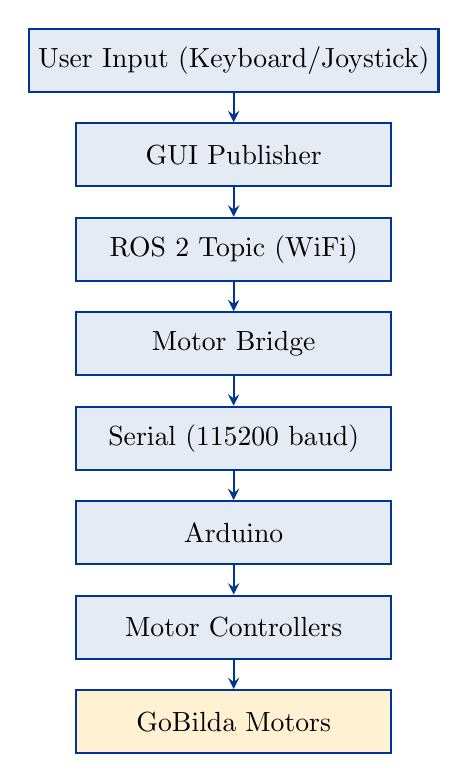
\begin{tikzpicture}[
    node distance=1.2cm,
    box/.style={rectangle, draw=pittblue, thick, minimum width=4cm, minimum height=0.8cm, align=center, fill=pittblue!10},
    arrow/.style={->, thick, >=stealth, pittblue}
]
    \node[box] (input) {User Input (Keyboard/Joystick)};
    \node[box, below of=input] (pub) {GUI Publisher};
    \node[box, below of=pub] (topic) {ROS 2 Topic (WiFi)};
    \node[box, below of=topic] (bridge) {Motor Bridge};
    \node[box, below of=bridge] (serial) {Serial (115200 baud)};
    \node[box, below of=serial] (arduino) {Arduino};
    \node[box, below of=arduino] (controller) {Motor Controllers};
    \node[box, below of=controller, fill=pittgold!20] (motors) {GoBilda Motors};

    \draw[arrow] (input) -- (pub);
    \draw[arrow] (pub) -- (topic);
    \draw[arrow] (topic) -- (bridge);
    \draw[arrow] (bridge) -- (serial);
    \draw[arrow] (serial) -- (arduino);
    \draw[arrow] (arduino) -- (controller);
    \draw[arrow] (controller) -- (motors);
\end{tikzpicture}
\caption{Motor Control Communication Flow}
\end{figure}

\section{Bidirectional Data Flow}

The system supports bidirectional communication: commands flow from the base station to the rover, while sensor data flows from the rover back to the base station.

\begin{figure}[H]
\centering
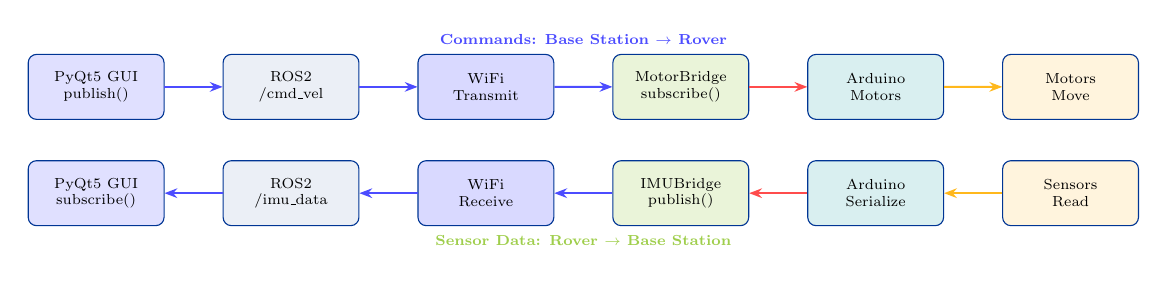
\begin{tikzpicture}[
    scale=0.75,
    transform shape,
    box/.style={rectangle, rounded corners=3pt, draw=pittblue, fill=pittblue!8, minimum width=2.3cm, minimum height=1.1cm, font=\scriptsize, align=center},
    arr/.style={-{Stealth[scale=0.7]}, thick},
]

% Commands flow (top)
\node[box, fill=blue!12] (gui) at (0,0.9) {PyQt5 GUI\\publish()};
\node[box] (ros1) at (3.3,0.9) {ROS2\\/cmd\_vel};
\node[box, fill=blue!15] (wifi1) at (6.6,0.9) {WiFi\\Transmit};
\node[box, fill=jetsongreen!15] (bridge1) at (9.9,0.9) {MotorBridge\\subscribe()};
\node[box, fill=arduinoblue!15] (ard1) at (13.2,0.9) {Arduino\\Motors};
\node[box, fill=pittgold!15] (hw1) at (16.5,0.9) {Motors\\Move};

\draw[arr, blue!70] (gui) -- (ros1);
\draw[arr, blue!70] (ros1) -- (wifi1);
\draw[arr, blue!70] (wifi1) -- (bridge1);
\draw[arr, red!70] (bridge1) -- (ard1);
\draw[arr, pittgold] (ard1) -- (hw1);

\node[font=\scriptsize\bfseries, blue!70] at (8.25,1.7) {Commands: Base Station $\rightarrow$ Rover};

% Sensor data flow (bottom)
\node[box, fill=pittgold!15] (hw2) at (16.5,-0.9) {Sensors\\Read};
\node[box, fill=arduinoblue!15] (ard2) at (13.2,-0.9) {Arduino\\Serialize};
\node[box, fill=jetsongreen!15] (bridge2) at (9.9,-0.9) {IMUBridge\\publish()};
\node[box, fill=blue!15] (wifi2) at (6.6,-0.9) {WiFi\\Receive};
\node[box] (ros2) at (3.3,-0.9) {ROS2\\/imu\_data};
\node[box, fill=blue!12] (gui2) at (0,-0.9) {PyQt5 GUI\\subscribe()};

\draw[arr, pittgold] (hw2) -- (ard2);
\draw[arr, red!70] (ard2) -- (bridge2);
\draw[arr, blue!70] (bridge2) -- (wifi2);
\draw[arr, blue!70] (wifi2) -- (ros2);
\draw[arr, blue!70] (ros2) -- (gui2);

\node[font=\scriptsize\bfseries, jetsongreen!70] at (8.25,-1.7) {Sensor Data: Rover $\rightarrow$ Base Station};

\end{tikzpicture}
\caption{Bidirectional Data Flow}
\label{fig:data-flow}
\end{figure}

%=============================================================================
\chapter{Directory Structure}
%=============================================================================

\section{Project Layout}

The project follows a modular organization:

\begin{lstlisting}[language=bash, caption={Project Directory Structure}]
URC/
|-- docker/                    # Docker configuration
|   |-- jetson/               # On-board Jetson container
|   |   |-- Dockerfile
|   |   |-- docker-compose.yml
|   |   |-- start.sh
|   |   |-- supervisord.conf
|   |   +-- setup.py
|   |-- jetson_local/         # Alternative Jetson setup
|   +-- local/                # Base station container
|       |-- Dockerfile
|       |-- docker-compose.yml
|       |-- start_mac.sh
|       |-- start_linux.sh
|       +-- sim-launch.sh
|
|-- ros_bridge/               # ROS 2 hardware bridges
|   |-- arduino_bridge_base/  # Base class for bridges
|   |-- motor_bridge/         # Motor control system
|   |-- motor_subscriber/     # Motor command handler
|   |-- gps_bridge/           # GPS sensor bridge
|   |-- imu_bridge/           # IMU sensor bridge
|   +-- ultrasonic_bridge/    # Ultrasonic sensor bridge
|
|-- guis/                     # PyQt5 GUI applications
|   |-- gen_gui.py            # Main control dashboard
|   |-- arduino_gui.py        # Hardware control interface
|   |-- auto_gui.py           # Autonomous navigation
|   |-- json_motorGUI.py      # Motor/Arm keyboard control
|   |-- publishers/           # ROS 2 publisher classes
|   |-- subscribers/          # ROS 2 subscriber classes
|   +-- camera/               # Camera utilities
|
|-- teleop/                   # Teleoperation system
|   +-- teleop_string_publisher.py
|
|-- odometry/                 # Navigation and localization
|   +-- gps/                  # GPS odometry utilities
|
|-- simulation/               # Gazebo simulation
|   +-- colcon_ws/            # ROS 2 workspace
|       +-- src/my_robot_description/
|
|-- README.md
|-- CONTRIBUTING.md
+-- Makefile
\end{lstlisting}

\section{Key Directories}

\subsection{Docker Configuration}

\begin{itemize}
    \item \texttt{docker/jetson/} --- On-board rover container with NVIDIA runtime support
    \item \texttt{docker/local/} --- Base station container with X11 forwarding for GUI
    \item \texttt{docker/jetson\_local/} --- Alternative hybrid setup
\end{itemize}

\subsection{ROS Bridge}

\begin{itemize}
    \item \texttt{arduino\_bridge\_base/} --- Base class providing serial communication (248 lines)
    \item \texttt{motor\_bridge/} --- Unified motor control with multiple input sources
    \item \texttt{gps\_bridge/} --- NMEA sentence parsing and publishing
    \item \texttt{imu\_bridge/} --- BNO055 9-axis IMU integration
    \item \texttt{ultrasonic\_bridge/} --- Multi-sensor distance measurement
\end{itemize}

\subsection{GUI System}

\begin{itemize}
    \item \texttt{gen\_gui.py} --- Main dashboard (623 lines) with camera feeds and sensor data
    \item \texttt{arduino\_gui.py} --- Joystick-style motor control (617 lines)
    \item \texttt{json\_motorGUI.py} --- Keyboard hotkey control (292 lines)
    \item \texttt{publishers/} --- MotorPublisher, TwistPublisher classes
    \item \texttt{subscribers/} --- IMUSubscriber, GPSSubscriber, data parsers
\end{itemize}

\section{Module Interdependencies}

Understanding how modules depend on each other helps developers know which files to modify when extending the system.

\subsection{Class Inheritance Hierarchy}

\begin{figure}[H]
\centering
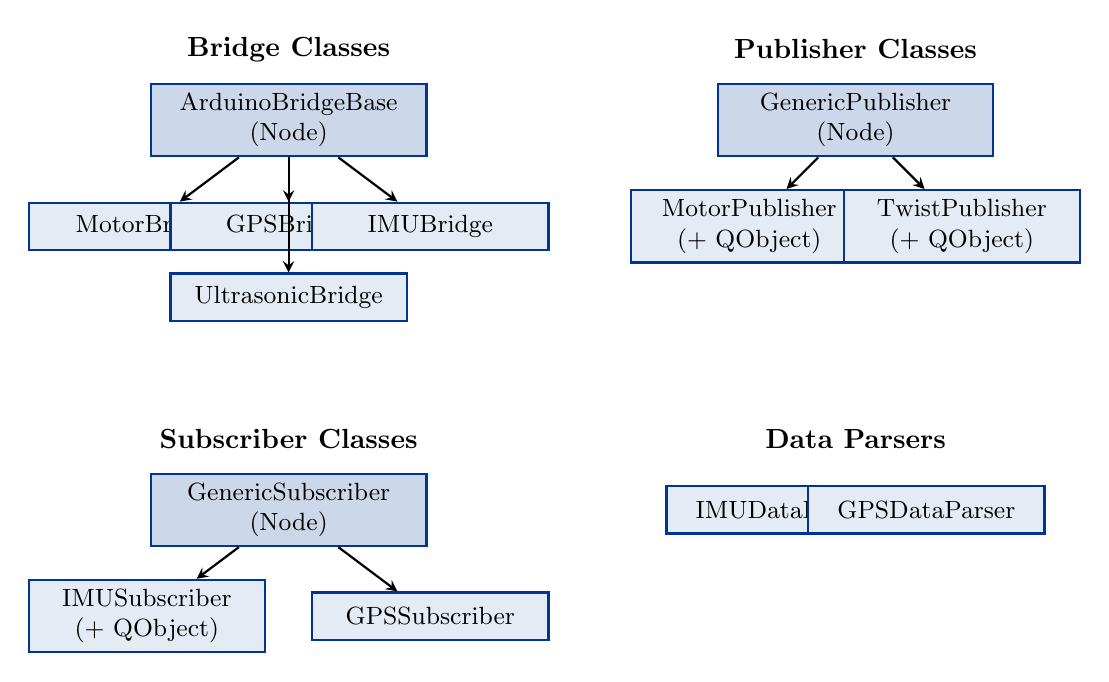
\begin{tikzpicture}[
    scale=0.9,
    node distance=1cm,
    base/.style={rectangle, draw=pittblue, thick, minimum width=3.5cm, minimum height=0.7cm, align=center, fill=pittblue!20, font=\small},
    child/.style={rectangle, draw=pittblue, thick, minimum width=3cm, minimum height=0.6cm, align=center, fill=pittblue!10, font=\small},
    arrow/.style={->, thick, >=stealth}
]
    % Bridge Hierarchy
    \node at (-4, 4) {\textbf{Bridge Classes}};
    \node[base] (bridgebase) at (-4, 3) {ArduinoBridgeBase\\(Node)};
    \node[child] (motor) at (-6, 1.5) {MotorBridge};
    \node[child] (gps) at (-4, 1.5) {GPSBridge};
    \node[child] (imu) at (-2, 1.5) {IMUBridge};
    \node[child] (ultra) at (-4, 0.5) {UltrasonicBridge};

    \draw[arrow] (bridgebase) -- (motor);
    \draw[arrow] (bridgebase) -- (gps);
    \draw[arrow] (bridgebase) -- (imu);
    \draw[arrow] (bridgebase) -- (ultra);

    % Publisher Hierarchy
    \node at (4, 4) {\textbf{Publisher Classes}};
    \node[base] (pubbase) at (4, 3) {GenericPublisher\\(Node)};
    \node[child] (motorpub) at (2.5, 1.5) {MotorPublisher\\(+ QObject)};
    \node[child] (twistpub) at (5.5, 1.5) {TwistPublisher\\(+ QObject)};

    \draw[arrow] (pubbase) -- (motorpub);
    \draw[arrow] (pubbase) -- (twistpub);

    % Subscriber Hierarchy
    \node at (-4, -1.5) {\textbf{Subscriber Classes}};
    \node[base] (subbase) at (-4, -2.5) {GenericSubscriber\\(Node)};
    \node[child] (imusub) at (-6, -4) {IMUSubscriber\\(+ QObject)};
    \node[child] (gpssub) at (-2, -4) {GPSSubscriber};

    \draw[arrow] (subbase) -- (imusub);
    \draw[arrow] (subbase) -- (gpssub);

    % Data Parser (standalone)
    \node at (4, -1.5) {\textbf{Data Parsers}};
    \node[child] (imuparse) at (3, -2.5) {IMUDataParser};
    \node[child] (gpsparse) at (5, -2.5) {GPSDataParser};

\end{tikzpicture}
\caption{Module Inheritance and Composition}
\end{figure}

\subsection{Import Dependencies}

\begin{table}[H]
\centering
\caption{Module Import Requirements}
\begin{tabular}{@{}lp{8cm}@{}}
\toprule
\textbf{Module} & \textbf{Key Imports} \\
\midrule
ArduinoBridgeBase & \texttt{rclpy}, \texttt{serial}, \texttt{std\_msgs.msg.String} \\
MotorBridge & ArduinoBridgeBase, \texttt{geometry\_msgs.msg.Twist} \\
GenericPublisher & \texttt{rclpy.node.Node} \\
MotorPublisher & GenericPublisher, \texttt{PyQt5.QtCore.QObject}, \texttt{pyqtSignal} \\
GenericSubscriber & \texttt{rclpy.node.Node} \\
IMUSubscriber & GenericSubscriber, IMUDataParser, \texttt{PyQt5.QtCore} \\
GPSSubscriber & GenericSubscriber, GPSDataParser \\
\bottomrule
\end{tabular}
\end{table}

\subsection{sys.path Configuration}

GUI modules require path configuration to import sibling packages:

\begin{lstlisting}[language=python, caption={Import Path Setup (from gen\_gui.py)}]
import sys
import os

# Add parent directory to path for sibling imports
sys.path.append(os.path.dirname(os.path.dirname(os.path.abspath(__file__))))

# Now can import from publishers/ and subscribers/
from guis.publishers.publisher import MotorPublisher
from guis.subscribers.subscriber import IMUSubscriber
\end{lstlisting}

\begin{tipbox}
\textbf{When adding new modules:}
\begin{itemize}
    \item Place publishers in \texttt{guis/publishers/} and inherit from \texttt{GenericPublisher}
    \item Place subscribers in \texttt{guis/subscribers/} and inherit from \texttt{GenericSubscriber}
    \item Place bridges in \texttt{ros\_bridge/<bridge\_name>/} and inherit from \texttt{ArduinoBridgeBase}
    \item Data parsers are standalone classes in \texttt{guis/subscribers/}
\end{itemize}
\end{tipbox}

%=============================================================================
\chapter{Hardware Requirements}
%=============================================================================

\section{Power System}

The rover uses a distributed power architecture with isolated rails for compute and motor systems.

\begin{table}[H]
\centering
\caption{Power System Specifications}
\begin{tabular}{@{}llp{6cm}@{}}
\toprule
\textbf{Component} & \textbf{Specification} & \textbf{Purpose} \\
\midrule
Batteries & 4$\times$ 40V rechargeable & Main power source for entire rover \\
Voltage Regulator \#1 & 40V $\rightarrow$ 5V & Dedicated power for Jetson Nano \\
Voltage Regulator \#2 & 40V $\rightarrow$ motor voltage & Powers motor controllers \\
Emergency Stop & Relay cutoff switch & Immediately disconnects all power \\
Power Distribution & Central module & Routes power to subsystems \\
\bottomrule
\end{tabular}
\end{table}

\begin{importantbox}
The power system uses \textbf{isolated power rails} to prevent motor inrush current from causing brownouts on the Jetson Nano. Voltage Regulator \#1 provides dedicated, stable power to the compute unit.
\end{importantbox}

\section{On-Board Computer}

\begin{table}[H]
\centering
\caption{Jetson Nano Specifications}
\begin{tabular}{@{}ll@{}}
\toprule
\textbf{Component} & \textbf{Specification} \\
\midrule
Computer & NVIDIA Jetson Nano (4GB) \\
Storage & 64GB+ SD Card or NVMe SSD \\
Power & 5V 4A barrel jack \\
Cooling & Active fan (recommended) \\
\bottomrule
\end{tabular}
\end{table}

\section{Motor System}

The motor system uses 6$\times$ GoBilda motors with 3 dual H-bridge controllers. For complete specifications, see the Key Specifications table in Chapter~\ref{chap:overview} and the Hardware Subsystems table in Chapter~\ref{chap:architecture}.

\subsection{Pin Configuration}

\begin{table}[H]
\centering
\caption{Arduino Motor Pin Configuration}
\begin{tabular}{@{}lccl@{}}
\toprule
\textbf{Motor} & \textbf{PWM Pin} & \textbf{Direction Pin} & \textbf{Side} \\
\midrule
Front Left & 2 & 53 & Left \\
Middle Left & 4 & 51 & Left \\
Back Left & 6 & 49 & Left \\
Front Right & 3 & 52 & Right \\
Middle Right & 5 & 50 & Right \\
Back Right & 7 & 48 & Right \\
\bottomrule
\end{tabular}
\end{table}

\section{Sensors}

\begin{table}[H]
\centering
\caption{Sensor Configuration}
\begin{tabular}{@{}lllc@{}}
\toprule
\textbf{Sensor} & \textbf{Model} & \textbf{Connection} & \textbf{Rate} \\
\midrule
IMU & Adafruit BNO055 (9-axis) & I2C via Arduino & 10 Hz \\
GPS & u-blox ZED-F9P RTK ($\pm$2cm) & Serial 115200 & 1 Hz \\
Cameras & 3$\times$ Intel RealSense D400 & USB 3.0 & 30 Hz \\
Ultrasonic & 3$\times$ HC-SR04 & Arduino GPIO & 10 Hz \\
\bottomrule
\end{tabular}
\end{table}

\subsection{Sensor Details}

\begin{itemize}
    \item \textbf{RTK GPS (ZED-F9P):} Uses carrier phase measurements instead of code-based positioning, achieving $\pm$2cm accuracy vs $\pm$5m standard GPS. Requires base station corrections.
    \item \textbf{IMU (BNO055):} 9-axis sensor (3-axis accelerometer, gyroscope, magnetometer) with onboard sensor fusion. Connected via I2C to dedicated Arduino.
    \item \textbf{Cameras (RealSense D400):} RGB-D cameras providing both color and depth data. Mounted at front, back, and on the robotic arm for manipulation tasks.
    \item \textbf{Ultrasonic (HC-SR04):} 3 sensors for obstacle detection. Range: 2cm--400cm. Pin configuration: Sensor 1 (Trigger=8, Echo=9), Sensor 2 (Trigger=50, Echo=51), Sensor 3 (Trigger=48, Echo=49).
\end{itemize}

\section{Serial Port Configuration}

\begin{table}[H]
\centering
\caption{Serial Port Assignments --- Port numbers depend on USB plug-in order (see Section~\ref{sec:usb-enumeration})}
\begin{tabular}{@{}lllll@{}}
\toprule
\textbf{Device} & \textbf{Port} & \textbf{Baud Rate} & \textbf{Arduino} & \textbf{Notes} \\
\midrule
Motors & /dev/ttyACM1 & 115200 & Hardcoded in motor\_subscriber \\
GPS & /dev/ttyACM0 & 9600 & SoftwareSerial (RX=10, TX=11) \\
IMU & TCP:8888 or Serial & 115200 & TCP in Docker, serial standalone \\
Ultrasonic & /dev/ttyACM0 & 115200 & Shared with GPS/IMU Arduino \\
\bottomrule
\end{tabular}
\end{table}

\begin{importantbox}
\textbf{IMU Communication Options:} The IMU bridge supports two modes:
\begin{itemize}
    \item \textbf{TCP Mode (Docker):} Connects to \texttt{host.docker.internal:8888} for use inside containers
    \item \textbf{Serial Mode (Standalone):} Auto-detects from \texttt{/dev/ttyACM0}, \texttt{/dev/ttyUSB0}, or \texttt{/dev/cu.usbmodem*}
\end{itemize}
\end{importantbox}

%=============================================================================
\chapter{Software Dependencies}
%=============================================================================

\section{System Requirements}

\begin{itemize}
    \item \textbf{Operating System:} Ubuntu 22.04 LTS
    \item \textbf{ROS Version:} ROS 2 Humble Hawksbill
    \item \textbf{Python:} 3.10+
    \item \textbf{Docker:} 20.10+
\end{itemize}

\section{Python Dependencies}

\begin{lstlisting}[language=bash, caption={Python Package Requirements}]
# Core ROS 2
rclpy
ros2cli

# Hardware Communication
pyserial>=3.5
pyrealsense2>=2.50.0

# GUI Framework
PyQt5>=5.15.0
PyQt5-sip

# Computer Vision
opencv-python>=4.5.0
numpy<2.0

# ROS 2 Message Bridges
cv_bridge
sensor_msgs
geometry_msgs
std_msgs
\end{lstlisting}

\section{System Packages (APT)}

\begin{lstlisting}[language=bash, caption={System Package Requirements}]
# Base development
python3-pip python3-pyqt5 python3-pyqt5.qtsvg

# Graphics libraries (for GUI)
libxcb-xinerama0 libxcb-cursor0 libxkbcommon-x11-0
libgl1-mesa-glx libgl1-mesa-dri mesa-utils x11-apps

# ROS 2 Humble
ros-humble-desktop ros-dev-tools
ros-humble-teleop-twist-keyboard ros-humble-joy

# Intel RealSense
librealsense2-utils librealsense2-dev
ros-humble-librealsense2-* ros-humble-realsense2-*
\end{lstlisting}

\section{Arduino Libraries}

\begin{itemize}
    \item \texttt{Adafruit\_Sensor} --- Unified sensor abstraction layer
    \item \texttt{Adafruit\_BNO055} --- 9-axis IMU driver library
\end{itemize}

\section{Dependency Rationale}

Understanding why each dependency is required helps developers troubleshoot installation issues and evaluate alternatives.

\begin{table}[H]
\centering
\caption{Python Package Rationale}
\begin{tabular}{@{}lllp{5cm}@{}}
\toprule
\textbf{Package} & \textbf{Version} & \textbf{Used By} & \textbf{Why Required} \\
\midrule
pyserial & $\geq$3.5 & ArduinoBridgeBase & Serial communication with Arduino; 3.5+ includes stability fixes for Linux \\
pyrealsense2 & $\geq$2.50.0 & setup.py, ImageSubscriber & Intel RealSense SDK bindings; 2.50+ required for D435 depth camera \\
PyQt5 & $\geq$5.15.0 & All GUIs & Qt bindings for GUI framework; 5.15+ has stable signal/slot mechanism \\
opencv-python & $\geq$4.5.0 & Camera utilities & Image processing and cv\_bridge integration \\
numpy & $<$2.0 & IMUDataParser, cameras & Matrix operations; 2.0 has breaking API changes affecting cv\_bridge \\
\bottomrule
\end{tabular}
\end{table}

\subsection{Version Constraint Explanations}

\begin{importantbox}
\textbf{numpy$<$2.0 Constraint}

NumPy 2.0 introduced breaking changes to array handling that affect \texttt{cv\_bridge} and OpenCV integration. The constraint is enforced in both Dockerfiles:

\begin{lstlisting}[language=bash]
# From docker/jetson/Dockerfile and docker/local/Dockerfile
RUN pip3 install 'numpy<2.0' opencv-python
\end{lstlisting}

If you upgrade to numpy 2.0+, expect \texttt{TypeError} exceptions when converting ROS Image messages to OpenCV arrays.
\end{importantbox}

\subsection{ROS 2 Humble Compatibility}

ROS 2 Humble (May 2022 -- May 2027) is the current LTS release. Key compatibility notes:

\begin{itemize}
    \item \textbf{Python 3.10+} --- Required by Humble; earlier Python versions will fail
    \item \textbf{Ubuntu 22.04} --- Official supported platform for Humble
    \item \textbf{DDS Implementation} --- Uses Fast-RTPS by default (\texttt{RMW\_IMPLEMENTATION=rmw\_fastrtps\_cpp})
\end{itemize}

\subsection{Development vs. Production Dependencies}

\begin{table}[H]
\centering
\caption{Dependency Categories}
\begin{tabular}{@{}llp{6cm}@{}}
\toprule
\textbf{Category} & \textbf{Packages} & \textbf{Notes} \\
\midrule
Core (Required) & rclpy, pyserial, PyQt5 & Essential for all operations \\
Sensors & pyrealsense2, Adafruit libraries & Only needed with corresponding hardware \\
Development & ros-dev-tools, x11-apps & Debugging and testing tools \\
Simulation & Gazebo packages & Only for simulation mode \\
\bottomrule
\end{tabular}
\end{table}

%=============================================================================
\chapter{Docker Configuration}
%=============================================================================

\section{Jetson Container}

\subsection{Overview}

The Jetson container runs on-board the rover and manages all hardware interfaces.

\begin{warningbox}
\textbf{CRITICAL: Re-Plug Arduinos Before EVERY Docker Start}

The Docker container captures serial port mappings at startup. You \textbf{MUST} unplug and re-plug the Arduinos in the correct order \textbf{every time} before starting the container:
\begin{enumerate}
    \item Unplug all Arduinos from Jetson
    \item Plug in \textbf{Sensor Arduino FIRST} $\rightarrow$ gets \texttt{/dev/ttyACM0}
    \item Plug in \textbf{Motor Arduino SECOND} $\rightarrow$ gets \texttt{/dev/ttyACM1}
    \item Verify with \texttt{ls /dev/ttyACM*}
    \item \textbf{Then} start the Docker container
\end{enumerate}
See Section~\ref{sec:usb-enumeration} for details.
\end{warningbox}

\begin{lstlisting}[language=bash, caption={Build and Start Jetson Container}]
cd docker/jetson
sudo docker build -t urc_jetson .
# FIRST: Re-plug Arduinos in correct order (Sensor, then Motor)
sudo docker-compose up -d
\end{lstlisting}

\subsection{Key Features}

\begin{itemize}
    \item NVIDIA GPU support (\texttt{runtime: nvidia})
    \item Privileged mode for device access
    \item Host network mode for ROS 2 communication
    \item Supervisor process management
\end{itemize}

\subsection{Device Mappings}

\begin{lstlisting}[language=yaml, caption={Docker Compose Device Configuration}]
devices:
  - /dev:/dev                    # All devices
  - /dev/bus/usb:/dev/bus/usb    # USB devices
  - /dev/video0:/dev/video0      # Camera 1
  - /dev/video1:/dev/video1      # Camera 2
\end{lstlisting}

\subsection{Environment Variables}

See Appendix~\ref{app:env-vars} for the complete environment variable reference. Key variables for Jetson include \texttt{ROS\_DOMAIN\_ID}, \texttt{NVIDIA\_DRIVER\_CAPABILITIES}, and \texttt{NVIDIA\_VISIBLE\_DEVICES}.

\subsection{Supervised Processes}

\begin{table}[H]
\centering
\caption{Supervisor Managed Processes}
\begin{tabular}{@{}llc@{}}
\toprule
\textbf{Process} & \textbf{Description} & \textbf{Auto-restart} \\
\midrule
setup & RealSense camera initialization & Yes \\
gps\_bridge & GPS data publisher & Yes \\
motor\_subscriber & Motor command handler & Yes \\
imu\_bridge & IMU orientation publisher & Yes \\
ultrasonic\_bridge & Ultrasonic sensor publisher & Yes \\
\bottomrule
\end{tabular}
\end{table}

\section{Local Container (Base Station)}

\subsection{macOS Setup}

\begin{lstlisting}[language=bash, caption={macOS Container Startup}]
# Prerequisite: Install XQuartz and enable network clients
# System Preferences > Security > Allow connections

cd docker/local
chmod +x start_mac.sh
./start_mac.sh
\end{lstlisting}

\subsection{Linux Setup}

\begin{lstlisting}[language=bash, caption={Linux Container Startup}]
cd docker/local
chmod +x start_linux.sh
./start_linux.sh
\end{lstlisting}

\subsection{Local Environment Variables}

See Appendix~\ref{app:env-vars} for the complete environment variable reference. Key variables for GUI display include \texttt{DISPLAY} and \texttt{QT\_X11\_NO\_MITSHM}.

\section{Simulation Container}

The simulation uses Gazebo with a custom URDF robot model.

\subsection{Simulation Workspace Structure}

\begin{lstlisting}[language=bash]
simulation/colcon_ws/
+-- src/
    +-- my_robot_description/
        |-- launch/
        |   |-- display.launch.py    # RViz visualization
        |   +-- launch_sim.launch.py # Full Gazebo simulation
        |-- urdf/
        |   +-- RAS_Rover.urdf       # Robot description
        +-- scripts/
            +-- robot_controller.py  # Simulation control
\end{lstlisting}

\subsection{Building the Simulation}

\begin{lstlisting}[language=bash, caption={Build Simulation Workspace}]
cd simulation/colcon_ws
colcon build --symlink-install
source install/setup.bash
\end{lstlisting}

\subsection{Launching Simulation}

\begin{lstlisting}[language=bash, caption={Simulation Startup}]
# Option 1: Via Docker
cd docker/local
./sim-launch.sh

# Option 2: Direct launch for RViz visualization
ros2 launch my_robot_description display.launch.py

# Option 3: Full Gazebo simulation
ros2 launch my_robot_description launch_sim.launch.py use_sim_time:=true
\end{lstlisting}

%=============================================================================
\chapter{Quick Start Guide}
%=============================================================================

\begin{tipbox}
This chapter provides a condensed overview of the startup process. For comprehensive step-by-step procedures, troubleshooting, and verification commands, see Chapter~\ref{chap:detailed-startup}: \textbf{Detailed Startup Procedures}.
\end{tipbox}

\section{Prerequisites}

\begin{warningbox}
\textbf{Linux Base Station Required:} To communicate with the rover Jetson, you must use a Linux-based base station. This can be:
\begin{itemize}
    \item A laptop or desktop running Linux (Ubuntu 22.04 recommended)
    \item Another Jetson device running the \texttt{jetson\_local} configuration
\end{itemize}
macOS support is limited to simulation and local development only.
\end{warningbox}

\subsection{Install Docker}

\begin{lstlisting}[language=bash, caption={Docker Installation}]
# Linux
curl -fsSL https://get.docker.com -o get-docker.sh
sudo sh get-docker.sh

# macOS
brew install --cask docker
\end{lstlisting}

\subsection{Clone Repository}

\begin{lstlisting}[language=bash, caption={Clone Repository}]
git clone https://github.com/pitt-robotics/URC.git
cd URC
\end{lstlisting}

\subsection{Connect Hardware}

\begin{warningbox}
\textbf{USB Connection Order is Critical!} The motor Arduino is hardcoded to \texttt{/dev/ttyACM1}. Linux assigns device numbers in the order USB devices are plugged in.
\end{warningbox}

\begin{enumerate}
    \item \textbf{First:} Plug in IMU/GPS Arduino (gets \texttt{/dev/ttyACM0})
    \item \textbf{Second:} Plug in Motor Arduino (gets \texttt{/dev/ttyACM1})
    \item Connect RealSense cameras to USB 3.0 ports
    \item Power on motor controllers
    \item Verify serial ports: \texttt{ls /dev/ttyACM*} (should show ACM0 and ACM1)
\end{enumerate}

\subsection{Network Setup}

\begin{enumerate}
    \item Connect the rover (Jetson) to the team WiFi network
    \item Connect the base station (Linux laptop/Jetson) to the \textbf{same WiFi network}
    \item Verify connectivity: \texttt{ping <rover-ip-address>}
\end{enumerate}

\begin{tipbox}
\textbf{Why This Matters:} Docker captures the \texttt{/dev/ttyACM*} mappings when the container starts. The MotorBridge is hardcoded to use \texttt{/dev/ttyACM1}, so the Motor Arduino \textbf{must} be the second device plugged in.
\end{tipbox}

\section{Option A: Full System Startup}

\begin{importantbox}
This option requires both the rover (Jetson) and base station (local machine) to be on the same WiFi network. The base station \textbf{must be running Linux} to communicate with the rover---use a Linux laptop or another Jetson with \texttt{jetson\_local}.
\end{importantbox}

\subsection{Step 1: Start Jetson Container (on rover)}

\begin{warningbox}
\textbf{Before running start.sh:} Unplug and re-plug Arduinos in correct order (Sensor first $\rightarrow$ ACM0, Motor second $\rightarrow$ ACM1). The container captures port assignments at startup!
\end{warningbox}

\begin{lstlisting}[language=bash]
# FIRST: Re-plug Arduinos (Sensor, then Motor)
cd docker/jetson
sudo ./start.sh
\end{lstlisting}

Enter the container and start the ROS bridges:

\begin{lstlisting}[language=bash]
# Enter the container
sudo docker exec -it pitt_urc_jetson bash

# Source ROS 2
source /opt/ros/humble/local_setup.bash
cd /app

# Start bridges (run each in separate terminal or use screen/tmux)
python3 -m ros_bridge.motor_subscriber.motor_subscriber
python3 -m ros_bridge.gps_bridge.gps_bridge
python3 -m ros_bridge.ultrasonic_bridge.ultrasonic_bridge
\end{lstlisting}

\subsection{Step 2: Start Local Container (on base station)}

\begin{lstlisting}[language=bash]
# macOS
cd docker/local
./start_mac.sh

# Linux
cd docker/local
./start_linux.sh
\end{lstlisting}

\subsection{Step 3: Launch GUI}

\begin{lstlisting}[language=bash]
# Inside local container
source /opt/ros/humble/local_setup.bash
cd /app
python3 -m guis.gen_gui
\end{lstlisting}

%=============================================================================
\chapter{Detailed Startup Procedures}
\label{chap:detailed-startup}
%=============================================================================

\section{Prerequisites}

\begin{warningbox}
\textbf{Linux Base Station Required:} To communicate with the rover Jetson, you must use a Linux-based base station. This can be a laptop running Linux (Ubuntu 22.04 recommended) or another Jetson device running the \texttt{jetson\_local} configuration.
\end{warningbox}

\subsection{USB Connection Order}

\begin{warningbox}
\textbf{USB Connection Order is Critical!} The motor Arduino is hardcoded to \texttt{/dev/ttyACM1}. Linux assigns device numbers in the order USB devices are plugged in.
\end{warningbox}

\begin{enumerate}
    \item \textbf{First:} Plug in IMU/GPS Arduino (gets \texttt{/dev/ttyACM0})
    \item \textbf{Second:} Plug in Motor Arduino (gets \texttt{/dev/ttyACM1})
    \item Connect RealSense cameras to USB 3.0 ports
    \item Power on motor controllers
    \item Verify serial ports: \texttt{ls /dev/ttyACM*} (should show ACM0 and ACM1)
\end{enumerate}

\subsection{Network Setup}

\begin{enumerate}
    \item Connect the rover (Jetson) to the team WiFi network
    \item Connect the base station (Linux laptop/Jetson) to the \textbf{same WiFi network}
    \item Verify connectivity: \texttt{ping <rover-ip-address>}
\end{enumerate}

\section{Jetson On-Board Startup}

\begin{lstlisting}[language=bash, caption={Complete Jetson Startup Procedure}]
# 1. SSH into Jetson
ssh nvidia@<jetson-ip>

# 2. Navigate to project
cd /path/to/URC

# 3. Build and start container (first time)
cd docker/jetson
sudo docker build -t urc_jetson .
sudo docker-compose up -d

# 4. Verify container is running
sudo docker ps

# 5. Enter the container
sudo docker exec -it pitt_urc_jetson bash

# 6. Source ROS 2 and navigate to app
source /opt/ros/humble/local_setup.bash
cd /app

# 7. Start ROS bridges (run each in separate terminal or use screen/tmux)
python3 -m ros_bridge.motor_subscriber.motor_subscriber
python3 -m ros_bridge.gps_bridge.gps_bridge
python3 -m ros_bridge.ultrasonic_bridge.ultrasonic_bridge
\end{lstlisting}

\section{Base Station Startup}

\subsection{macOS Procedure}

\begin{lstlisting}[language=bash, caption={macOS Base Station Startup}]
# 1. Start XQuartz
open -a XQuartz

# 2. Enable network clients (if not done)
# XQuartz > Preferences > Security > Allow connections

# 3. Navigate to project
cd /path/to/URC/docker/local

# 4. Start container
./start_mac.sh

# 5. Source ROS 2
source /opt/ros/humble/local_setup.bash

# 6. Launch main GUI
cd /app
python3 -m guis.gen_gui
\end{lstlisting}

\subsection{Linux Procedure}

\begin{lstlisting}[language=bash, caption={Linux Base Station Startup}]
# 1. Navigate to project
cd /path/to/URC/docker/local

# 2. Start container
./start_linux.sh

# 3. Source ROS 2
source /opt/ros/humble/local_setup.bash

# 4. Launch main GUI
cd /app
python3 -m guis.gen_gui
\end{lstlisting}

\section{Verification Steps}

\subsection{Check ROS 2 Connectivity}

\begin{lstlisting}[language=bash, caption={ROS 2 Verification Commands}]
# List all active nodes
ros2 node list

# Expected:
# /motor_subscriber
# /gps_bridge
# /imu_bridge
# /ultrasonic_bridge

# List all topics
ros2 topic list

# Expected:
# /cmd_vel
# /motor_control_input
# /drive_data
# /gps_data
# /imu_data
# /ultrasonic_data
# /camera/gray/image_raw
# /camera/depth/image_raw
\end{lstlisting}

\subsection{Test Motor Commands}

\begin{warningbox}
Be careful when testing motor commands! Ensure the rover is in a safe position before sending movement commands.
\end{warningbox}

\begin{lstlisting}[language=bash, caption={Motor Command Testing}]
# Send stop command
ros2 topic pub --once /motor_control_input std_msgs/String \
    "data: '0,0,0,0,0,0'"

# Send forward command (be careful!)
ros2 topic pub --once /motor_control_input std_msgs/String \
    "data: '100,0,0,0,0,0'"
\end{lstlisting}

\subsection{Monitor Sensor Data}

\begin{lstlisting}[language=bash, caption={Sensor Data Monitoring}]
# IMU data
ros2 topic echo /imu_data

# GPS data
ros2 topic echo /gps_data

# Ultrasonic data
ros2 topic echo /ultrasonic_data
\end{lstlisting}

%=============================================================================
\chapter{ROS 2 Architecture}
%=============================================================================

\section{Node Overview}

\begin{table}[H]
\centering
\caption{ROS 2 Nodes}
\begin{tabular}{@{}llp{6cm}@{}}
\toprule
\textbf{Node} & \textbf{Package} & \textbf{Purpose} \\
\midrule
motor\_bridge & ros\_bridge & Motor command handling and feedback \\
gps\_bridge & ros\_bridge & GPS NMEA data publishing \\
imu\_bridge & ros\_bridge & IMU orientation data publishing \\
ultrasonic\_bridge & ros\_bridge & Distance measurement publishing \\
gray\_and\_depth\_publisher & guis.camera & Camera feed publishing \\
\bottomrule
\end{tabular}
\end{table}

\section{Topic Architecture}

\begin{figure}[H]
\centering
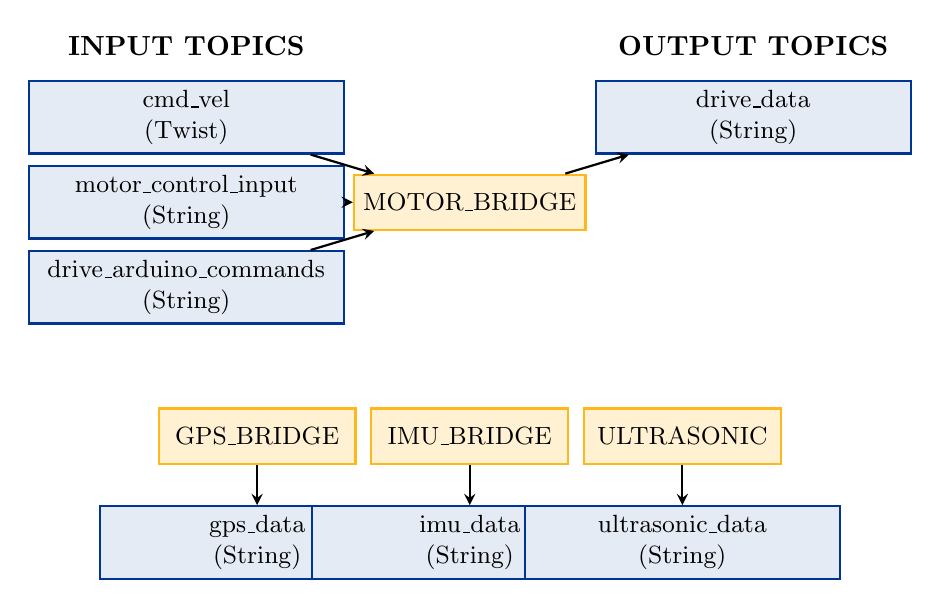
\begin{tikzpicture}[
    scale=0.9,
    node distance=0.8cm,
    topicbox/.style={rectangle, draw=pittblue, thick, minimum width=4cm, minimum height=0.7cm, align=center, fill=pittblue!10, font=\small},
    nodebox/.style={rectangle, draw=pittgold, thick, minimum width=2.5cm, minimum height=0.7cm, align=center, fill=pittgold!20, font=\small},
    arrow/.style={->, thick, >=stealth}
]
    % Input Topics
    \node at (-4, 5) {\textbf{INPUT TOPICS}};
    \node[topicbox] (cmdvel) at (-4, 4) {cmd\_vel\\(Twist)};
    \node[topicbox] (motor) at (-4, 2.8) {motor\_control\_input\\(String)};
    \node[topicbox] (legacy) at (-4, 1.6) {drive\_arduino\_commands\\(String)};

    % Motor Bridge
    \node[nodebox] (motorbridge) at (0, 2.8) {MOTOR\_BRIDGE};

    % Output Topics
    \node at (4, 5) {\textbf{OUTPUT TOPICS}};
    \node[topicbox] (drivedata) at (4, 4) {drive\_data\\(String)};

    % Sensor Bridges
    \node[nodebox] (gpsbridge) at (-3, -0.5) {GPS\_BRIDGE};
    \node[nodebox] (imubridge) at (0, -0.5) {IMU\_BRIDGE};
    \node[nodebox] (ultrabridge) at (3, -0.5) {ULTRASONIC};

    % Sensor Topics
    \node[topicbox] (gpsdata) at (-3, -2) {gps\_data\\(String)};
    \node[topicbox] (imudata) at (0, -2) {imu\_data\\(String)};
    \node[topicbox] (ultradata) at (3, -2) {ultrasonic\_data\\(String)};

    % Arrows
    \draw[arrow] (cmdvel) -- (motorbridge);
    \draw[arrow] (motor) -- (motorbridge);
    \draw[arrow] (legacy) -- (motorbridge);
    \draw[arrow] (motorbridge) -- (drivedata);

    \draw[arrow] (gpsbridge) -- (gpsdata);
    \draw[arrow] (imubridge) -- (imudata);
    \draw[arrow] (ultrabridge) -- (ultradata);

\end{tikzpicture}
\caption{ROS 2 Topic Architecture}
\end{figure}

\section{Message Formats}

\begin{importantbox}
\textbf{Motor Control: Two Input Methods}

The motor bridge accepts commands from two different topic types:
\begin{itemize}
    \item \texttt{/cmd\_vel} (geometry\_msgs/Twist) --- Standard ROS 2 velocity commands. Used by teleop\_twist\_keyboard, joystick drivers, and autonomous navigation nodes.
    \item \texttt{/motor\_control\_input} (std\_msgs/String) --- Direct 6-value control. Used by custom GUIs for fine-grained motor testing.
\end{itemize}
Both are converted to PWM signals by the MotorBridge. Use \texttt{/cmd\_vel} for standard robot control; use \texttt{/motor\_control\_input} for direct hardware testing.
\end{importantbox}

\subsection{Motor Control Input (String)}

\begin{lstlisting}[caption={Motor Command Format}]
Format: "linear_x,linear_y,linear_z,angular_x,angular_y,angular_z"
Example: "100,0,0,0,0,50"  # Forward with slight right turn
\end{lstlisting}

\subsection{IMU Data (String)}

\begin{lstlisting}[caption={IMU Data Format}]
Format: "X: <value>\tY: <value>\tZ: <value>"
Example: "X: 0.123\tY: 0.456\tZ: 0.789"
\end{lstlisting}

\subsection{GPS Data (String)}

\begin{lstlisting}[caption={GPS NMEA Format}]
NMEA sentences:
$GNGLL,4024.12345,N,07952.12345,W,123456.00,A,A*6B
$GAGSV,3,1,12,01,45,123,38,02,67,234,42,...
\end{lstlisting}

\subsection{Ultrasonic Data (String)}

\begin{lstlisting}[caption={Ultrasonic Data Format}]
Format: "distance1_cm, distance2_cm, distance3_cm, "
Example: "45, 120, 88, "
\end{lstlisting}

%=============================================================================
\chapter{Hardware Interfaces}
%=============================================================================

\section{Motor Control}

\subsection{Arduino Firmware}

\textbf{Location:} \texttt{ros\_bridge/motor\_subscriber/motor\_serial/motor\_serial.ino}

\begin{lstlisting}[language=C, caption={Motor Control Logic}]
// Simplified differential drive
left_speed = linear_x - angular_z;
right_speed = linear_x + angular_z;

// PWM mapping
pwm_left = map(left_speed, -100, 100, -255, 255);
pwm_right = map(right_speed, -100, 100, -255, 255);

// Direction Control
// HIGH = Forward
// LOW = Reverse
\end{lstlisting}

\section{IMU (BNO055)}

\textbf{Location:} \texttt{ros\_bridge/imu\_bridge/imu\_serial/imu\_serial.ino}

\begin{lstlisting}[language=C, caption={IMU Configuration}]
Adafruit_BNO055 bno = Adafruit_BNO055(55);
bno.setExtCrystalUse(true);  // External crystal for accuracy

// Output Format
Serial.print("X: "); Serial.print(event.orientation.x);
Serial.print("\tY: "); Serial.print(event.orientation.y);
Serial.print("\tZ: "); Serial.println(event.orientation.z);
\end{lstlisting}

\subsection{Data Processing}

\begin{lstlisting}[language=python, caption={IMU Data Parser}]
# IMUDataParser.py
import math

distance = math.sqrt(
    (x_cur - x_prev)**2 +
    (y_cur - y_prev)**2 +
    (z_cur - z_prev)**2
)
velocity = distance / time_delta
vertical_tilt = math.degrees(math.atan2(y_delta, z_delta))
horizontal_tilt = math.degrees(math.atan2(y_delta, x_delta))
\end{lstlisting}

\section{GPS}

\textbf{Location:} \texttt{ros\_bridge/gps\_bridge/gps/gps.ino}

\begin{table}[H]
\centering
\caption{NMEA Sentence Types}
\begin{tabular}{@{}ll@{}}
\toprule
\textbf{Type} & \textbf{Purpose} \\
\midrule
GNGLL & Geographic position (latitude/longitude) \\
GAGSV & GPS satellites in view + SNR \\
GBGSV & BeiDou satellites in view + SNR \\
\bottomrule
\end{tabular}
\end{table}

\section{Ultrasonic Sensors}

\textbf{Location:} \texttt{ros\_bridge/ultrasonic\_bridge/multiple\_ultrasonic\_sensors/}

\begin{lstlisting}[language=C, caption={Ultrasonic Distance Calculation}]
duration = pulseIn(echoPin, HIGH);
distance_cm = (duration / 2) / 29.1;
\end{lstlisting}

\section{RealSense Cameras}

\textbf{Location:} \texttt{guis/camera/camera\_cv\_test.py}

The rover uses Intel RealSense D435 RGB-D cameras for vision and depth sensing.

\subsection{Camera Specifications}

\begin{table}[H]
\centering
\caption{RealSense D435 Configuration}
\begin{tabular}{@{}lll@{}}
\toprule
\textbf{Stream} & \textbf{Resolution} & \textbf{Format} \\
\midrule
Color & 640$\times$480 @ 30 FPS & BGR8 \\
Depth & 640$\times$480 @ 30 FPS & Z16 (16-bit depth) \\
Grayscale & 640$\times$480 @ 30 FPS & MONO8 (converted) \\
\bottomrule
\end{tabular}
\end{table}

\subsection{Published Topics}

\begin{table}[H]
\centering
\caption{Camera ROS Topics}
\begin{tabular}{@{}lll@{}}
\toprule
\textbf{Topic} & \textbf{Message Type} & \textbf{Description} \\
\midrule
/camera/gray/image\_raw & sensor\_msgs/Image & Grayscale image (mono8) \\
/camera/depth/image\_raw & sensor\_msgs/Image & Depth image (16UC1) \\
\bottomrule
\end{tabular}
\end{table}

\subsection{Configuration Code}

\begin{lstlisting}[language=python, caption={RealSense Configuration}]
import pyrealsense2 as rs

# Initialize pipeline
pipeline = rs.pipeline()
config = rs.config()

# Color stream (converted to grayscale for publishing)
config.enable_stream(rs.stream.color, 640, 480, rs.format.bgr8, 30)

# Depth stream
config.enable_stream(rs.stream.depth, 640, 480, rs.format.z16, 30)

# Start streaming
pipeline.start(config)
\end{lstlisting}

\begin{tipbox}
The camera publisher converts color frames to grayscale before publishing to reduce bandwidth. Connect cameras to USB 3.0 ports for optimal performance.
\end{tipbox}

%=============================================================================
\chapter{GUI System}
\label{chap:gui-system}
%=============================================================================

\section{Main Control GUI}

\textbf{File:} \texttt{guis/gen\_gui.py} (623 lines)

\begin{table}[H]
\centering
\caption{Main GUI Components}
\begin{tabular}{@{}lp{8cm}@{}}
\toprule
\textbf{Section} & \textbf{Function} \\
\midrule
Title Bar & Connection status (ONLINE/OFFLINE) \\
Navigation Tabs & Switch between competition modes \\
Camera Feeds & 3 video displays (primary, secondary, auxiliary) \\
IMU Display & Speed, vertical tilt, horizontal tilt \\
System Controls & Toggle IMU, GPS, orientation \\
Emergency Stop & Red button for immediate halt \\
\bottomrule
\end{tabular}
\end{table}

\begin{lstlisting}[language=bash, caption={Launch Main GUI}]
python3 -m guis.gen_gui
\end{lstlisting}

\section{Motor/Arm GUI Hotkeys}

\textbf{File:} \texttt{guis/json\_motorGUI.py} (292 lines)

\begin{table}[H]
\centering
\caption{Motor Control Hotkeys}
\begin{tabular}{@{}cl@{}}
\toprule
\textbf{Key} & \textbf{Action} \\
\midrule
I & Forward \\
, (comma) & Backward \\
L & Turn Right \\
J & Turn Left \\
Q & Speed Up \\
Z & Slow Down \\
K & Stop \\
\bottomrule
\end{tabular}
\end{table}

\begin{table}[H]
\centering
\caption{Arm Control Hotkeys}
\begin{tabular}{@{}cl@{}}
\toprule
\textbf{Key} & \textbf{Action} \\
\midrule
0/9 & Claw open/close \\
M/N & Base shift right/left \\
U/J & Bottom joint forward/backward \\
I/K & Middle joint forward/backward \\
O/L & Top joint forward/backward \\
Y/H & Wrist clockwise/counterclockwise \\
Escape & Emergency stop all \\
\bottomrule
\end{tabular}
\end{table}

\begin{warningbox}
\textbf{Keybinding Conflict Warning}

The \texttt{json\_motorGUI.py} Motor and Arm windows share overlapping key bindings that cause conflicts when both windows are open:

\begin{center}
\begin{tabular}{@{}ccc@{}}
\toprule
\textbf{Key} & \textbf{Motor Action} & \textbf{Arm Action} \\
\midrule
I & Forward & Middle joint forward \\
J & Turn left & Bottom joint backward \\
K & Stop & Middle joint backward \\
L & Turn right & Top joint backward \\
\bottomrule
\end{tabular}
\end{center}

\textbf{Recommendation:} Only open one control window at a time, or modify keybindings in the source code to eliminate conflicts.
\end{warningbox}

\section{Alternative GUI: HTTP-Based Control (json\_motorGUI.py)}

\textbf{Location:} \texttt{guis/json\_motorGUI.py}

\begin{importantbox}
\textbf{Different Communication Architecture}

Unlike the main GUIs that use ROS 2, the \texttt{json\_motorGUI.py} uses HTTP POST requests to communicate with a local server. This requires a separate HTTP server running on \texttt{localhost:8000}.
\end{importantbox}

\textbf{Architecture:}
\begin{enumerate}
    \item GUI sends HTTP POST to \texttt{http://localhost:8000/}
    \item JSON payload contains command code: \texttt{\{"rover": 1\}} or \texttt{\{"arm": 0\}}
    \item HTTP server (not included) must translate commands to motor/arm control
\end{enumerate}

\textbf{Command Codes:}

\begin{table}[H]
\centering
\caption{Rover HTTP Command Codes}
\begin{tabular}{@{}clc@{}}
\toprule
\textbf{Code} & \textbf{Action} & \textbf{JSON Payload} \\
\midrule
1 & Forward & \texttt{\{"rover": 1\}} \\
2 & Reverse & \texttt{\{"rover": 2\}} \\
3 & Turn Left & \texttt{\{"rover": 3\}} \\
4 & Turn Right & \texttt{\{"rover": 4\}} \\
5 & Speed Up (Boost) & \texttt{\{"rover": 5\}} \\
6 & Slow Down & \texttt{\{"rover": 6\}} \\
7 & Stop & \texttt{\{"rover": 7\}} \\
\bottomrule
\end{tabular}
\end{table}

\begin{table}[H]
\centering
\caption{Arm HTTP Command Codes}
\begin{tabular}{@{}clc@{}}
\toprule
\textbf{Code} & \textbf{Action} & \textbf{JSON Payload} \\
\midrule
0 & Claw Open & \texttt{\{"arm": 0\}} \\
1 & Claw Close & \texttt{\{"arm": 1\}} \\
2 & Base Shift Right & \texttt{\{"arm": 2\}} \\
3 & Base Shift Left & \texttt{\{"arm": 3\}} \\
4 & Bottom Joint Forward & \texttt{\{"arm": 4\}} \\
5 & Bottom Joint Reverse & \texttt{\{"arm": 5\}} \\
6 & Middle Joint Forward & \texttt{\{"arm": 6\}} \\
7 & Middle Joint Reverse & \texttt{\{"arm": 7\}} \\
8 & Top Joint Forward & \texttt{\{"arm": 8\}} \\
9 & Top Joint Reverse & \texttt{\{"arm": 9\}} \\
10 & Wrist Clockwise & \texttt{\{"arm": 10\}} \\
11 & Wrist Counterclockwise & \texttt{\{"arm": 11\}} \\
12 & Stop All & \texttt{\{"arm": 12\}} \\
\bottomrule
\end{tabular}
\end{table}

\begin{warningbox}
\textbf{HTTP Server Requirement}

The \texttt{json\_motorGUI.py} will fail with connection errors if no HTTP server is running on port 8000. This GUI is designed for use with a custom HTTP-to-serial bridge that is separate from the ROS 2 infrastructure.
\end{warningbox}

\section{ROS 2 Motor Control GUI (arduino\_gui.py)}

\textbf{Location:} \texttt{guis/arduino\_gui.py}

This GUI uses ROS 2 for motor control (unlike \texttt{json\_motorGUI.py}).

\textbf{Key Features:}
\begin{itemize}
    \item \textbf{ThrottleControl Widget} --- Custom QFrame with slider (0-100\%), reset/full buttons
    \item \textbf{Physics Simulation} --- Acceleration/deceleration at 20 FPS (50ms timer)
    \item \textbf{WASD Controls} --- Hold SHIFT + direction keys to apply throttle
    \item \textbf{ROS 2 Integration} --- Publishes to \texttt{motor\_control\_input} topic via MotorPublisher
\end{itemize}

\textbf{Keybindings (arduino\_gui.py):}
\begin{table}[H]
\centering
\begin{tabular}{@{}cl@{}}
\toprule
\textbf{Key} & \textbf{Action} \\
\midrule
W & Forward (with SHIFT held) \\
S & Backward (with SHIFT held) \\
A & Turn Left (with SHIFT held) \\
D & Turn Right (with SHIFT held) \\
SHIFT & Apply throttle (hold to accelerate) \\
SPACE & Emergency brake (immediate stop) \\
\bottomrule
\end{tabular}
\end{table}

\textbf{Physics Parameters:}
\begin{lstlisting}[language=python, caption={Physics Constants in arduino\_gui.py}]
self.acceleration_rate = 0.1      # Rate toward target speed
self.deceleration_rate = 0.08     # Rate when releasing throttle
self.angular_deceleration_rate = 0.1
# Angular velocity decay multiplier: 0.7 (applied per frame)
# Physics update rate: 50ms (20 FPS)
\end{lstlisting}

\section{Publisher Classes}

\textbf{Location:} \texttt{guis/publishers/publisher.py}

\begin{lstlisting}[language=python, caption={MotorPublisher Class}]
class MotorPublisher(GenericPublisher):
    def __init__(self):
        super().__init__('motor_control_input', String)

    def publish_motor_command(self, motor_values):
        # motor_values: list of 6 floats
        msg = String()
        msg.data = ','.join(map(str, motor_values))
        self.publisher.publish(msg)

    def stop_all_motors(self):
        self.publish_motor_command([0, 0, 0, 0, 0, 0])
\end{lstlisting}

\begin{lstlisting}[language=python, caption={TwistPublisher Class}]
class TwistPublisher(GenericPublisher):
    def __init__(self):
        super().__init__('cmd_vel', Twist)

    def move_forward(self, speed):
        msg = Twist()
        msg.linear.x = float(speed)
        self.publisher.publish(msg)

    def turn_left(self, angular_speed):
        msg = Twist()
        msg.angular.z = float(angular_speed)
        self.publisher.publish(msg)
\end{lstlisting}

\section{Event Handling Architecture}

The GUI system uses PyQt5's signal/slot mechanism to safely communicate between ROS 2 threads and the GUI thread.

\subsection{Signal/Slot Pattern}

ROS 2 callbacks execute in separate threads, but Qt GUI updates must happen in the main thread. Signals bridge this gap:

\begin{lstlisting}[language=python, caption={Signal Definition and Emission}]
# In IMUSubscriber (guis/subscribers/subscriber.py)
class IMUSubscriber(GenericSubscriber, QObject):
    # Define signal with parameter types
    imu_data_updated = pyqtSignal(float, float, float)

    def default_callback(self, msg):
        # Parse data in ROS thread
        parsed_data = self.parser.parse_imu_data(msg.data)
        self.velocity, self.vertical_tilt, self.horizontal_tilt = parsed_data[1:4]

        # Emit signal (thread-safe crossing to GUI thread)
        self.imu_data_updated.emit(
            self.velocity,
            self.vertical_tilt,
            self.horizontal_tilt
        )
\end{lstlisting}

\begin{lstlisting}[language=python, caption={Signal Connection in GUI}]
# In MainWindow (guis/gen_gui.py)
def setup_subscribers(self):
    self.imu_subscriber = IMUSubscriber()

    # Connect signal to slot (GUI update method)
    self.imu_subscriber.imu_data_updated.connect(self.update_imu_display)

def update_imu_display(self, velocity, vert_tilt, horiz_tilt):
    # This runs in GUI thread - safe to update widgets
    self.speed_label.setText(f"{velocity:.2f} m/s")
    self.vert_tilt_label.setText(f"{vert_tilt:.1f} deg")
    self.horiz_tilt_label.setText(f"{horiz_tilt:.1f} deg")
\end{lstlisting}

\subsection{Available Signals}

\begin{table}[H]
\centering
\caption{PyQt5 Signals in the System}
\begin{tabular}{@{}llp{5cm}@{}}
\toprule
\textbf{Class} & \textbf{Signal} & \textbf{Parameters} \\
\midrule
IMUSubscriber & imu\_data\_updated & (float, float, float) --- velocity, vert\_tilt, horiz\_tilt \\
MotorPublisher & message\_published & (str) --- the published command string \\
TwistPublisher & twist\_published & (float $\times$ 6) --- linear xyz, angular xyz \\
\bottomrule
\end{tabular}
\end{table}

\subsection{Keyboard Event Handling}

The \texttt{json\_motorGUI.py} implements keyboard control using Qt's \texttt{keyPressEvent}:

\begin{lstlisting}[language=python, caption={Keyboard Control Pattern}]
# Command codes (from json_motorGUI.py lines 9-30)
FORWARD = 1
REVERSE = 2
LEFT = 3
RIGHT = 4
SPEED_UP = 5
SLOW_DOWN = 6
STOP = 7

class MotorWindow(QWidget):
    def keyPressEvent(self, event):
        key = event.key()

        if key == Qt.Key_I:
            self.send_command(FORWARD)
        elif key == Qt.Key_Comma:
            self.send_command(REVERSE)
        elif key == Qt.Key_J:
            self.send_command(LEFT)
        elif key == Qt.Key_L:
            self.send_command(RIGHT)
        elif key == Qt.Key_K:
            self.send_command(STOP)
        elif key == Qt.Key_Escape:
            self.emergency_stop()
\end{lstlisting}

\section{Extending the GUI System}

\subsection{Adding a New Sensor Display}

To add a new sensor type to the GUI:

\begin{enumerate}
    \item \textbf{Create Data Parser} (if needed) in \texttt{guis/subscribers/}
    \item \textbf{Create Subscriber Class} inheriting from \texttt{GenericSubscriber}
    \item \textbf{Define PyQt Signal} with appropriate parameter types
    \item \textbf{Connect Signal to Slot} in your GUI class
    \item \textbf{Create UI Widgets} to display the data
\end{enumerate}

\begin{lstlisting}[language=python, caption={Example: Adding Temperature Sensor Display}]
# 1. Create TempSubscriber in guis/subscribers/subscriber.py
class TempSubscriber(GenericSubscriber, QObject):
    temp_updated = pyqtSignal(float)  # temperature in Celsius

    def __init__(self):
        super().__init__('temp_data', String, 'temp_subscriber')
        QObject.__init__(self)

    def default_callback(self, msg):
        temp = float(msg.data)
        self.temp_updated.emit(temp)

# 2. In your GUI class
self.temp_subscriber = TempSubscriber()
self.temp_subscriber.temp_updated.connect(self.update_temp_display)

def update_temp_display(self, temp):
    self.temp_label.setText(f"Temp: {temp:.1f} C")
\end{lstlisting}

\subsection{Adding a New Control Button}

To add a new control that sends commands to the rover:

\begin{lstlisting}[language=python, caption={Adding Custom Control Button}]
# In your GUI setup
self.custom_button = QPushButton("Custom Action")
self.custom_button.clicked.connect(self.on_custom_click)

# Create publisher instance
self.motor_pub = MotorPublisher()

def on_custom_click(self):
    # Send custom motor command
    self.motor_pub.publish_motor_command([50, 0, 0, 0, 0, 25])
\end{lstlisting}

%=============================================================================
\chapter{Development Workflow}
%=============================================================================

\section{Git Workflow}

\subsection{Branch Strategy}

\begin{itemize}
    \item \texttt{main} --- Protected, requires PR review
    \item \texttt{feature/*} --- New features
    \item \texttt{bugfix/*} --- Bug fixes
    \item \texttt{hotfix/*} --- Urgent production fixes
\end{itemize}

\subsection{Standard Workflow}

\begin{lstlisting}[language=bash, caption={Git Development Workflow}]
# 1. Fetch latest
git fetch origin

# 2. Create feature branch
git checkout -b feature/my-feature main

# 3. Make changes
# ... edit files ...

# 4. Stage and commit
git add .
git commit -m "feat: add my feature description"

# 5. Push to remote
git push origin feature/my-feature

# 6. Create Pull Request on GitHub
\end{lstlisting}

\subsection{Commit Message Format}

\begin{lstlisting}[caption={Commit Message Types}]
type: description

Types:
- feat: New feature
- fix: Bug fix
- docs: Documentation
- refactor: Code refactoring
- test: Testing
- chore: Maintenance
\end{lstlisting}

\section{Adding a New Sensor Bridge}

\subsection{Step 1: Create Arduino Firmware}

\begin{lstlisting}[language=C, caption={New Sensor Arduino Code}]
// ros_bridge/new_sensor_bridge/new_sensor_serial/new_sensor_serial.ino
void setup() {
    Serial.begin(115200);
}

void loop() {
    // Read sensor
    float value = readSensor();

    // Send data
    Serial.println(value);
    delay(100);
}
\end{lstlisting}

\subsection{Step 2: Create Python Bridge}

\begin{lstlisting}[language=python, caption={New Sensor Python Bridge}]
# ros_bridge/new_sensor_bridge/new_sensor_bridge.py
from ros_bridge.arduino_bridge_base.arduino_bridge_base import ArduinoBridgeBase
from std_msgs.msg import String

class NewSensorBridge(ArduinoBridgeBase):
    def __init__(self):
        super().__init__(
            node_name='new_sensor_bridge',
            topic_name='new_sensor_data',
            msg_type=String,
            serial_port='/dev/ttyACM0',
            baud_rate=115200
        )
\end{lstlisting}

\subsection{Step 3: Add to Supervisor}

\begin{lstlisting}[caption={Supervisor Configuration Entry}]
# docker/jetson/supervisord.conf
[program:new_sensor_bridge]
command=python3 /app/ros_bridge/new_sensor_bridge/new_sensor_bridge.py
stdout_logfile=/app/new_sensor_bridge.log
stderr_logfile=/app/new_sensor_bridge_err.log
autorestart=true
\end{lstlisting}

%=============================================================================
\chapter{Troubleshooting}
\label{chap:troubleshooting}
%=============================================================================

\begin{importantbox}
\textbf{\#1 Cause of System Failures: Arduino Plug-In Order}

Before troubleshooting anything else, verify:
\begin{enumerate}
    \item Did you \textbf{re-plug Arduinos before starting Docker}?
    \item Was \textbf{Sensor Arduino plugged in FIRST} (becomes \texttt{/dev/ttyACM0})?
    \item Was \textbf{Motor Arduino plugged in SECOND} (becomes \texttt{/dev/ttyACM1})?
\end{enumerate}

\textbf{Docker captures port mappings at startup.} If you started the container with Arduinos in the wrong order (or unplugged), the bridges will fail silently or connect to the wrong device.

\textbf{Quick Fix:} \texttt{docker-compose down} $\rightarrow$ unplug all $\rightarrow$ plug Sensor $\rightarrow$ plug Motor $\rightarrow$ \texttt{docker-compose up -d}

See Section~\ref{sec:usb-enumeration} for the complete USB Port Enumeration Order guide.
\end{importantbox}

\section{Common Issues}

\begin{longtable}{@{}p{3.5cm}p{4cm}p{5.5cm}@{}}
\toprule
\textbf{Issue} & \textbf{Cause} & \textbf{Solution} \\
\midrule
\endhead
Serial port not found & Device not connected or wrong plug-in order & Check USB connections, verify \texttt{/dev/ttyACM*} exists. \textbf{Ensure correct plug-in order} (see Section~\ref{sec:usb-enumeration}) \\
\midrule
Motors not responding & Wrong port, baud rate, or plug-in order & Motor Arduino must be \texttt{/dev/ttyACM1} (plugged in \textbf{second}). See Section~\ref{sec:usb-enumeration} for required order \\
\midrule
Sensor data missing & Wrong plug-in order & Sensor Arduino must be \texttt{/dev/ttyACM0} (plugged in \textbf{first}). See Section~\ref{sec:usb-enumeration} \\
\midrule
ROS topics not visible & Domain ID mismatch & Ensure \texttt{ROS\_DOMAIN\_ID=0} on both systems \\
\midrule
GUI won't display & X11 forwarding issue & Check \texttt{DISPLAY} variable, restart XQuartz \\
\midrule
Camera black screen & USB bandwidth & Use USB 3.0 ports, reduce resolution \\
\midrule
High latency & Network congestion & Check WiFi signal, reduce message frequency \\
\midrule
IMU returns -0.1 values & Parse error in IMUDataParser & Check serial format matches "X: val\textbackslash tY: val\textbackslash tZ: val", verify BNO055 calibration \\
\midrule
GPS shows "NO CONNECTION!!!" & Empty NMEA sentence & Check GPS serial connection, verify module has satellite fix \\
\midrule
Motor command ignored & Invalid 6-value format & Verify comma-separated format with no spaces, check for exactly 6 values \\
\midrule
Ultrasonic shows 0.0 & Sensor timeout or wiring & Check trigger/echo pin wiring, verify object is within sensor range (2-400cm) \\
\midrule
Qt platform plugin error & Missing X11 libraries & Install \texttt{libxcb-xinerama0}, restart container \\
\midrule
Camera black after restart & RealSense USB reset needed & Unplug/replug USB cable, run \texttt{rs-enumerate-devices} \\
\midrule
ROS nodes visible but no data & QoS mismatch & Ensure \texttt{queue\_size=10} on both publisher and subscriber \\
\midrule
Container exits immediately & Supervisor config error & Check \texttt{/app/*.log} files inside container for startup errors \\
\midrule
PyQt5 signal not received & Thread safety violation & Use \texttt{pyqtSignal} for cross-thread communication, never update GUI directly from ROS callback \\
\midrule
Serial permission denied & User not in dialout group & Run \texttt{sudo usermod -a -G dialout \$USER}, then logout/login \\
\bottomrule
\caption{Common Issues and Solutions}
\end{longtable}

\section{Docker Container Restart Guide}

When serial ports change (e.g., Arduino reconnected to different USB port), you must restart the Docker container to pick up the new device mapping.

\begin{importantbox}
\textbf{Key Concept: Docker Captures Ports at Startup}

The Docker container maps \texttt{/dev/ttyACM*} devices \textbf{only when it starts}. If you:
\begin{itemize}
    \item Unplug/replug an Arduino while the container is running $\rightarrow$ container won't see the change
    \item Start the container with Arduinos unplugged $\rightarrow$ container has no serial access
    \item Start the container with wrong plug-in order $\rightarrow$ ports are swapped, motors/sensors fail
\end{itemize}

\textbf{Solution:} Always re-plug Arduinos in correct order \textbf{before} every \texttt{docker-compose up}.
\end{importantbox}

\subsection{When to Restart}

\begin{itemize}
    \item Arduino disconnected and reconnected (port may change from \texttt{/dev/ttyACM0} to \texttt{/dev/ttyACM1})
    \item New USB device added that wasn't present at container start
    \item Serial permission changes made to host system
    \item After modifying \texttt{docker-compose.yml} device mappings
    \item \textbf{Every time you want fresh, correct serial port assignments}
\end{itemize}

\subsection{Complete Restart Procedure}

\begin{lstlisting}[language=bash, caption={Docker Container Restart for Port Changes}]
# 1. Stop the running container
cd docker/jetson  # or docker/local
sudo docker-compose down

# 2. RE-PLUG ARDUINOS IN CORRECT ORDER (CRITICAL!)
#    a. Unplug ALL Arduinos from Jetson
#    b. Wait 2 seconds
#    c. Plug in SENSOR Arduino FIRST -> becomes /dev/ttyACM0
#    d. Wait 2 seconds
#    e. Plug in MOTOR Arduino SECOND -> becomes /dev/ttyACM1

# 3. Verify correct port assignments
ls -la /dev/ttyACM*
# MUST show: ttyACM0 (Sensor) and ttyACM1 (Motor)

# 4. (Optional) Update docker-compose.yml if needed
# Edit the devices section if needed:
#   devices:
#     - /dev/ttyACM0:/dev/ttyACM0
#     - /dev/ttyACM1:/dev/ttyACM1

# 5. Start the container (AFTER re-plugging Arduinos!)
sudo docker-compose up -d

# 6. Verify container is running and processes started
sudo docker ps
sudo docker exec -it pitt_urc_jetson supervisorctl status

# 7. Check bridge logs for serial connection success
sudo docker exec -it pitt_urc_jetson tail -f /app/motor_bridge.log
# Look for: "Serial connection established on /dev/ttyACM1"
\end{lstlisting}

\begin{warningbox}
\textbf{Port Hardcoding Warning}

The \texttt{MotorBridge} class has the serial port hardcoded to \texttt{/dev/ttyACM1}. If your Arduino appears on a different port, you have two options:

\begin{enumerate}
    \item \textbf{Create symlink on host} (recommended):
    \begin{lstlisting}[language=bash]
sudo ln -sf /dev/ttyACM0 /dev/ttyACM1
    \end{lstlisting}

    \item \textbf{Modify source code}:
    Edit \texttt{ros\_bridge/arduino\_bridge\_base/arduino\_bridge\_base.py} line 98:
    \begin{lstlisting}[language=python]
serial_port="/dev/ttyACM0",  # Change to your port
    \end{lstlisting}
\end{enumerate}
\end{warningbox}

\subsection{USB Port Enumeration Order}
\label{sec:usb-enumeration}

\begin{importantbox}
\textbf{Critical: Arduino Plug-In Order Matters}

The Jetson (and Linux in general) assigns serial port numbers based on the \textbf{order devices are plugged in}, not by physical USB port location. The first USB serial device plugged in becomes \texttt{/dev/ttyACM0}, the second becomes \texttt{/dev/ttyACM1}, and so on.
\end{importantbox}

\textbf{How Port Assignment Works:}

\begin{enumerate}
    \item When the Jetson boots with no USB devices connected, no \texttt{/dev/ttyACM*} ports exist
    \item The \textbf{first Arduino plugged in} is assigned \texttt{/dev/ttyACM0}
    \item The \textbf{second Arduino plugged in} is assigned \texttt{/dev/ttyACM1}
    \item If a device is unplugged and replugged, it may get a different port number
\end{enumerate}

\textbf{Required Plug-In Order for URC System:}

Based on the hardcoded port assignments in \texttt{arduino\_bridge\_base.py}:

\begin{center}
\begin{tabular}{@{}clll@{}}
\toprule
\textbf{Order} & \textbf{Arduino} & \textbf{Expected Port} & \textbf{Bridge Class} \\
\midrule
1st (plug in first) & Sensor Arduino (IMU/GPS/Ultrasonic) & \texttt{/dev/ttyACM0} & IMUBridge, GPSBridge, UltrasonicBridge \\
2nd (plug in second) & Motor Arduino & \texttt{/dev/ttyACM1} & MotorBridge \\
\bottomrule
\end{tabular}
\end{center}

\begin{lstlisting}[language=python, caption={Port Assignments in arduino\_bridge\_base.py}]
# MotorBridge - HARDCODED to ACM1 (line 98)
class MotorBridge(ArduinoBridgeBase):
    def __init__(self):
        super().__init__(
            serial_port="/dev/ttyACM1",  # Must be second device
            ...
        )

# Sensor bridges default to ACM0
class UltrasonicBridge(ArduinoBridgeBase):
    def __init__(self, serial_port="/dev/ttyACM0", ...):  # First device

class GPSBridge(ArduinoBridgeBase):
    def __init__(self, serial_port="/dev/ttyACM0", ...):  # First device

class IMUBridge(ArduinoBridgeBase):
    def __init__(self):
        possible_ports = ["/dev/ttyACM0", ...]  # Tries ACM0 first
\end{lstlisting}

\textbf{Startup Procedure:}

\begin{enumerate}
    \item Power on Jetson with \textbf{no Arduinos connected}
    \item Wait for Jetson to fully boot (login screen or SSH available)
    \item Plug in \textbf{Sensor Arduino first} (IMU/GPS/Ultrasonic) $\rightarrow$ becomes \texttt{/dev/ttyACM0}
    \item Plug in \textbf{Motor Arduino second} $\rightarrow$ becomes \texttt{/dev/ttyACM1}
    \item Verify ports with: \texttt{ls -la /dev/ttyACM*}
    \item Start Docker container: \texttt{sudo docker-compose up -d}
\end{enumerate}

\begin{warningbox}
\textbf{Common Mistake: Wrong Plug-In Order}

If you plug in the Motor Arduino first, it gets \texttt{/dev/ttyACM0} but the MotorBridge expects \texttt{/dev/ttyACM1}. Symptoms:
\begin{itemize}
    \item Motor commands have no effect
    \item Bridge logs show ``Serial connection established'' but motors don't respond
    \item IMU/GPS bridge fails to connect (expected port is taken by wrong Arduino)
\end{itemize}

\textbf{Fix:} Unplug both Arduinos, wait 2 seconds, then plug them in the correct order.
\end{warningbox}

\textbf{Verifying Correct Port Assignment:}

\begin{lstlisting}[language=bash, caption={Verify Arduino Port Assignment}]
# List connected serial devices
ls -la /dev/ttyACM*

# Expected output when correctly plugged in:
# /dev/ttyACM0 -> Sensor Arduino (first plugged in)
# /dev/ttyACM1 -> Motor Arduino (second plugged in)

# Check which Arduino is on which port by monitoring serial output:
# Terminal 1 - Monitor ACM0 (should show IMU/GPS data)
screen /dev/ttyACM0 115200

# Terminal 2 - Monitor ACM1 (should respond to motor commands)
screen /dev/ttyACM1 115200

# Exit screen: Ctrl+A, then K, then Y
\end{lstlisting}

\begin{tipbox}
\textbf{Pro Tip: udev Rules for Persistent Naming}

For production deployments, create udev rules to assign consistent device names based on hardware serial numbers instead of plug-in order:

\begin{lstlisting}[language=bash]
# Find Arduino serial number
udevadm info -a -n /dev/ttyACM0 | grep serial

# Create udev rule (as root)
echo 'SUBSYSTEM=="tty", ATTRS{serial}=="YOUR_SERIAL", SYMLINK+="arduino_motor"' \
    >> /etc/udev/rules.d/99-arduino.rules

# Reload rules
sudo udevadm control --reload-rules
\end{lstlisting}

Then update bridge code to use \texttt{/dev/arduino\_motor} instead of \texttt{/dev/ttyACM1}.
\end{tipbox}

\subsection{Quick Restart Commands}

\begin{warningbox}
\textbf{Remember:} Before ANY \texttt{docker-compose up} command, re-plug Arduinos in correct order!
\end{warningbox}

\begin{lstlisting}[language=bash, caption={Quick Restart Reference}]
# === BEFORE ANY RESTART: Re-plug Arduinos ===
# 1. Unplug all Arduinos
# 2. Plug Sensor Arduino (ACM0)
# 3. Plug Motor Arduino (ACM1)
# 4. Verify: ls /dev/ttyACM*

# Full restart (recommended for port changes)
sudo docker-compose down && sudo docker-compose up -d

# Restart single bridge process (port must be same - NO re-plug needed)
sudo docker exec -it pitt_urc_jetson supervisorctl restart motor_bridge

# Rebuild and restart (after code changes)
sudo docker-compose down
# Re-plug Arduinos here!
sudo docker build -t urc_jetson .
sudo docker-compose up -d

# Force recreate container (clears all state)
# Re-plug Arduinos first!
sudo docker-compose up -d --force-recreate
\end{lstlisting}

\section{Complete Cold-Start Procedure}

This section provides a comprehensive, step-by-step guide for starting the entire URC system from a powered-off state.

\begin{importantbox}
\textbf{Critical: Follow This Order Exactly}

The USB port enumeration is determined by plug-in order. Deviating from this procedure will result in incorrect port assignments and system failures.
\end{importantbox}

\subsection{Phase 1: Hardware Power-Up}

\begin{enumerate}
    \item \textbf{Ensure all Arduinos are UNPLUGGED} from the Jetson
    \item Power on the Jetson Nano
    \item Wait for complete boot (login prompt or SSH available) --- approximately 60-90 seconds
    \item Power on the base station computer
\end{enumerate}

\subsection{Phase 2: Arduino Connection (Critical Order)}

\begin{enumerate}
    \item \textbf{Plug in Sensor Arduino FIRST}
    \begin{itemize}
        \item This Arduino runs IMU, GPS, and ultrasonic firmware
        \item It will be assigned \texttt{/dev/ttyACM0}
        \item Wait 2 seconds for device enumeration
    \end{itemize}

    \item \textbf{Plug in Motor Arduino SECOND}
    \begin{itemize}
        \item This Arduino runs motor control firmware
        \item It will be assigned \texttt{/dev/ttyACM1}
        \item Wait 2 seconds for device enumeration
    \end{itemize}

    \item \textbf{Verify port assignments on Jetson:}
    \begin{lstlisting}[language=bash]
ls -la /dev/ttyACM*
# Expected output:
# /dev/ttyACM0 -> Sensor Arduino
# /dev/ttyACM1 -> Motor Arduino
    \end{lstlisting}
\end{enumerate}

\subsection{Phase 3: Start Jetson Container}

\begin{lstlisting}[language=bash, caption={Jetson Container Startup}]
# SSH into Jetson (or use direct terminal)
ssh user@jetson-ip

# Navigate to docker directory
cd ~/URC/docker/jetson

# Start container in detached mode
sudo docker-compose up -d

# Verify container is running
sudo docker ps
# Should show: pitt_urc_jetson

# Check Supervisor processes started
sudo docker exec -it pitt_urc_jetson supervisorctl status
# Expected: motor_bridge RUNNING, imu_bridge RUNNING, etc.

# Monitor bridge logs for serial connection success
sudo docker exec -it pitt_urc_jetson tail -f /app/motor_bridge.log
# Look for: "Serial connection established on /dev/ttyACM1"
\end{lstlisting}

\subsection{Phase 4: Start Base Station Container}

\begin{lstlisting}[language=bash, caption={Base Station Container Startup}]
# On base station computer
cd ~/URC/docker/local

# Start container
sudo docker-compose up -d

# Verify container
sudo docker ps
# Should show: pitt_urc_local
\end{lstlisting}

\subsection{Phase 5: Verify ROS 2 Communication}

\begin{lstlisting}[language=bash, caption={ROS 2 Verification}]
# On base station, enter container
sudo docker exec -it pitt_urc_local bash

# Source ROS 2
source /opt/ros/humble/local_setup.bash

# Check for topics from Jetson
ros2 topic list
# Expected: /imu_data, /gps_data, /motor_control_input, /cmd_vel, etc.

# Test IMU data reception
ros2 topic echo /imu_data
# Should show: data: "X: <val>\tY: <val>\tZ: <val>"

# Test motor command transmission
ros2 topic pub --once /motor_control_input std_msgs/String "data: '0,0,0,0,0,0'"
# Motors should remain stopped (all zeros)
\end{lstlisting}

\subsection{Phase 6: Launch GUI}

\begin{lstlisting}[language=bash, caption={GUI Launch}]
# Inside base station container
cd /app/guis

# Launch main GUI
python3 gen_gui.py

# OR launch motor control GUI (ROS 2 based)
python3 arduino_gui.py

# OR launch HTTP-based GUI (requires HTTP server)
# python3 json_motorGUI.py
\end{lstlisting}

\subsection{Verification Checklist}

\begin{table}[H]
\centering
\caption{Cold-Start Verification Checklist}
\begin{tabular}{@{}lcp{6cm}@{}}
\toprule
\textbf{Component} & \textbf{Status} & \textbf{Verification Command} \\
\midrule
Jetson booted & $\square$ & SSH connection successful \\
Sensor Arduino (ACM0) & $\square$ & \texttt{ls /dev/ttyACM0} exists \\
Motor Arduino (ACM1) & $\square$ & \texttt{ls /dev/ttyACM1} exists \\
Jetson container & $\square$ & \texttt{docker ps} shows running \\
Bridges running & $\square$ & \texttt{supervisorctl status} all RUNNING \\
Serial connected & $\square$ & Bridge logs show "established" \\
Base container & $\square$ & \texttt{docker ps} shows running \\
ROS topics visible & $\square$ & \texttt{ros2 topic list} shows topics \\
IMU data flowing & $\square$ & \texttt{ros2 topic echo /imu\_data} shows data \\
GUI launches & $\square$ & Window appears, no errors \\
\bottomrule
\end{tabular}
\end{table}

\begin{warningbox}
\textbf{Troubleshooting Cold-Start Failures}

\begin{itemize}
    \item \textbf{No /dev/ttyACM* devices:} Unplug both Arduinos, wait 5 seconds, replug in correct order
    \item \textbf{Bridge shows "Serial connection failed":} Wrong plug-in order. Restart from Phase 2
    \item \textbf{ROS topics not visible:} Check \texttt{ROS\_DOMAIN\_ID=0} on both systems
    \item \textbf{GUI crashes on launch:} Verify X11 forwarding (\texttt{echo \$DISPLAY} should be set)
    \item \textbf{Motors don't respond:} Verify Motor Arduino is on ACM1 (plug-in order issue)
\end{itemize}
\end{warningbox}

\section{Serial Port Debugging}

\begin{lstlisting}[language=bash, caption={Serial Port Debugging Commands}]
# List all serial ports
ls -la /dev/ttyACM* /dev/ttyUSB*

# Check port permissions
sudo chmod 666 /dev/ttyACM0

# Test serial communication
screen /dev/ttyACM0 115200

# Kill screen session: Ctrl+A, then K
\end{lstlisting}

\section{ROS 2 Debugging}

For ROS 2 debugging commands (checking environment, sourcing, discovery verification), see Appendix~\ref{app:commands}: Quick Command Reference.

\section{Docker Debugging}

\begin{lstlisting}[language=bash, caption={Docker Debugging Commands}]
# Check container status
docker ps -a

# View container logs
docker logs pitt_urc_jetson

# Enter running container
docker exec -it pitt_urc_jetson bash

# Check supervisor status (inside Jetson container)
supervisorctl status
supervisorctl restart motor_subscriber
\end{lstlisting}

\section{Log File Locations}

\begin{table}[H]
\centering
\caption{Log File Locations}
\begin{tabular}{@{}llp{5cm}@{}}
\toprule
\textbf{Log} & \textbf{Location} & \textbf{Content} \\
\midrule
Motor Bridge & /app/motor\_bridge.log & Motor commands, errors \\
GPS Bridge & /app/gps\_bridge.log & NMEA sentences \\
Ultrasonic & /app/ultrasonic\_bridge.log & Distance readings \\
Setup & /app/setup.log & Camera initialization \\
\bottomrule
\end{tabular}
\end{table}

%=============================================================================
\chapter{API Reference}
%=============================================================================

\section{ArduinoBridgeBase}

\begin{lstlisting}[language=python, caption={ArduinoBridgeBase API}]
class ArduinoBridgeBase(Node):
    """Base class for all Arduino serial bridges."""

    def __init__(self, node_name, topic_name, msg_type,
                 serial_port='/dev/ttyACM0', baud_rate=115200):
        """
        Initialize the bridge.

        Args:
            node_name: ROS 2 node name
            topic_name: Topic to publish/subscribe
            msg_type: ROS 2 message type (e.g., String)
            serial_port: Serial port path
            baud_rate: Baud rate (default: 115200)
        """

    def read_from_arduino(self):
        """Read data from Arduino and publish to ROS topic."""

    def write_to_arduino(self, data):
        """Write data to Arduino serial port."""
\end{lstlisting}

\begin{tipbox}
For MotorPublisher and TwistPublisher API documentation, see the Publisher Classes section in Chapter~\ref{chap:gui-system} (GUI System).
\end{tipbox}

%=============================================================================
% Appendices
%=============================================================================
\appendix

\chapter{Environment Variables}
\label{app:env-vars}

\begin{table}[H]
\centering
\caption{Environment Variable Reference}
\begin{tabular}{@{}llp{6cm}@{}}
\toprule
\textbf{Variable} & \textbf{Default} & \textbf{Description} \\
\midrule
ROS\_DOMAIN\_ID & 0 & ROS 2 domain for multi-device networking \\
ROS\_LOCALHOST\_ONLY & 0 & Allow network communication (0=yes, 1=no) \\
DISPLAY & :0 & X11 display for GUI \\
QT\_X11\_NO\_MITSHM & 1 & Qt X11 compatibility \\
NVIDIA\_VISIBLE\_DEVICES & all & GPU access (Jetson) \\
NVIDIA\_DRIVER\_CAPABILITIES & all & GPU capabilities (Jetson) \\
\bottomrule
\end{tabular}
\end{table}

\chapter{Quick Command Reference}
\label{app:commands}

\begin{lstlisting}[language=bash, caption={Quick Command Reference}]
# Docker
docker build -t urc_jetson .
docker-compose up -d
docker exec -it pitt_urc_jetson bash
docker logs pitt_urc_jetson

# ROS 2
source /opt/ros/humble/local_setup.bash
ros2 node list
ros2 topic list
ros2 topic echo /topic_name
ros2 topic pub --once /topic std_msgs/String "data: 'test'"

# GUI
python3 -m guis.gen_gui
python3 -m guis.arduino_gui
python3 -m guis.json_motorGUI

# Supervisor (inside Jetson container)
supervisorctl status
supervisorctl restart motor_subscriber
supervisorctl tail -f motor_subscriber

# Serial
ls /dev/ttyACM*
screen /dev/ttyACM0 115200
\end{lstlisting}

\chapter{Network Ports}

\begin{table}[H]
\centering
\caption{Network Port Reference}
\begin{tabular}{@{}lll@{}}
\toprule
\textbf{Port} & \textbf{Protocol} & \textbf{Service} \\
\midrule
7400 & UDP & ROS 2 DDS Discovery \\
8000 & HTTP & Motor/Arm GUI server \\
11311 & TCP & ROS Master (legacy) \\
\bottomrule
\end{tabular}
\end{table}

%=============================================================================
% Back matter
%=============================================================================

\chapter*{Document Information}
\addcontentsline{toc}{chapter}{Document Information}

\begin{table}[H]
\centering
\begin{tabular}{@{}ll@{}}
\toprule
\textbf{Field} & \textbf{Value} \\
\midrule
Document Version & 2.0 \\
Last Updated & January 2026 \\
Maintained by & University of Pittsburgh Robotics Club \\
Repository & github.com/pitt-robotics/URC \\
\bottomrule
\end{tabular}
\end{table}

\vspace{1cm}

For questions or contributions, please refer to \texttt{CONTRIBUTING.md} or open an issue on GitHub.

\end{document}
